% Correos y rutas largas de los instrumentos no se pueden cortar
\sloppy

\section{Soluciones existentes a Nixlang}\label{Appendix1}

\begin{table}[htbp]
\centering
\setlength{\tabcolsep}{4pt}
\begin{tabularx}{\textwidth}{|p{25pt}|X|X|X|X|}
\hline
 & \textbf{Problema} & \textbf{Soluciones} \newline \textbf{existentes} & \textbf{Limitaciones} & \textbf{Propuesta} \\
\hline
\cite{Courts2013} & Necesidad de aprender un lenguaje exclusivo de Nix & Uso de lenguajes de propósito general (e.g., Guile en Guix) & Lenguajes poco adoptados mantienen la barrera de entrada~\cite{stackoverflowMostPopularTechnologies} & Adoptar un lenguaje ampliamente conocido \\
\hline
\cite{gagarinFourMonthsNix} & Escasez de documentación y ejemplos & Reescritura de la documentación en un lugar centralizado & Alto costo de mantenimiento y dependencia de aprobación & Que la estructura del código en sí permite su documentación como el tipado estático \\
\hline
\cite{caddetNixNickel} \newline \cite{hufschmittCurrentStatePtyx} & Dependencia de funciones de la librería estándar con muchos parámetros no documentados. & Extensiones al lenguaje para tipado estático & Alta complejidad de implementación & Delegar el tipado a herramientas externas maduras \\
\hline
\cite{Schwaighofer2026} & Alta complejidad general del ecosistema & Generación de código con Inteligencia Artificial & No aborda causas estructurales; depende de datos de entrenamiento & Evitar soluciones basadas en generación automática \\
\hline
\end{tabularx}
\caption{Una tabla comparativa sobre algunas de las soluciones propuestas por la comunidad de Nix que buscan mejorar la experiencia en Nixlang de forma directa o indirecta, incluyendo sus limitaciones y una propuesta derivada.}
\end{table}

\section{Interés en Neovim}\label{Appendix2}

Con datos extraídos de Google Trends para la búsqueda ``Neovim - Programa'' en su modo clásico, se obtuvieron series históricas correspondientes a los últimos años. Los datos utilizados se muestran en~\cite{googleNeovimInterestTrends}.

\begin{figure}[htbp]
\centering
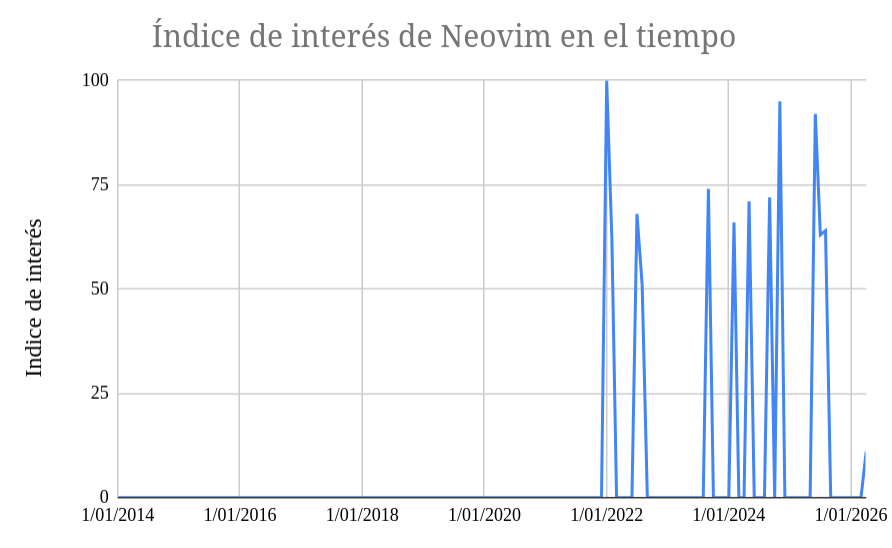
\includegraphics[width=0.74\textwidth]{anexo_interes_neovim.png}
\caption[Índice de interés de búsqueda de Neovim en Google entre 2014 y 2026. Se observa un aumento a finales de 2021, aproximadamente seis meses después de la introducción del soporte para Lua.]{Índice de interés de búsqueda de Neovim en Google entre 2014 y 2026. Se observa un aumento a finales de 2021, aproximadamente seis meses después de la introducción del soporte para Lua~\cite{NeovimNews112021}.}
\end{figure}

\section{Número de dependencias de Firefox}\label{Appendix5}

Con datos extraidos de Github del repositorio de \texttt{mozilla-\allowbreak{}firefox/\allowbreak{}firefox} para el commit \texttt{ac91bfcce1bf3240e2dce40f47c372e76bc4f26c} se descargaron las dependencias detectadas por Github en formato SBOM (estándar SPDX 2.3) en la sección de ``Grafo de Dependencias'', revelando una total de 22,732 dependencias. Los datos utilizados se encuentran en \texttt{2/\allowbreak{}mozilla-\allowbreak{}firefox\textunderscore{}\allowbreak{}dependencies.\allowbreak{}json}.

Del archivo SBOM se extrajeron 21,295 paquetes y 37,926 relaciones de dependencia directa (\texttt{DEPENDS\textunderscore{}ON})\footnote{La diferencia con las 22,732 dependencias reportadas por la interfaz de Github se debe a que, según indica el propio archivo, la versión exacta de algunos paquetes no pudo ser resuelta.}, que se usaron para construir un grafo de dependencias. Los dependencias son mostradas en la Figura~\ref{figure3}.

\section{Consentimientos Informados}

\subsection{Plantilla Fase 1}

\noindent
\begin{tabularx}{\linewidth}{@{}lX@{}}
\textbf{PROYECTO:} & \emph{Nix para todos: Impacto del uso de un lenguaje de propósito general en la usabilidad de Nix} \\[0.35em]
\textbf{Investigador:} & \emph{Daniel Alfredo Rayo Roldán - ray22933@uvg.edu.gt} \\[0.35em]
\textbf{Supervisor:} & \emph{Gabriel Brolo Tobar - gbrolo@uvg.edu.gt} \\
\end{tabularx}

\subsubsection{1. Introducción}

Gracias por considerar participar en nuestro estudio. Este formulario de consentimiento
informado tiene como objetivo proporcionarle información importante sobre el propósito, los
procedimientos y los posibles riesgos y beneficios de participar en este estudio. Por favor, lea
cuidadosamente este documento antes de aceptar participar. Si tiene alguna pregunta, no
dude en preguntar al investigador.

\subsubsection{2. Propósito del Estudio}

El propósito de este estudio es recopilar información sobre \textbf{la experiencia de uso en lenguajes de programación}.

La información obtenida en este estudio se utilizará para \textbf{comprender las necesidades y puntos de mejorar que tienen los lenguajes de configuración para administración de paquetes de \emph{software}}.

\subsubsection{3. Procedimientos del Estudio}

Si decide participar en este estudio, se le pedirá que \textbf{proporcione información sobre su experiencia general en desarrollo de software y administración de paquetes}.

El procedimiento tomará aproximadamente \textbf{2 hora y 30 minutos} para completarse y hará preguntas sobre \textbf{sobre como aprendes lenguajes de programación}.

La toma de muestra implicará \textbf{ver unos tutoriales de lenguajes de programación, para luego llenar un cuestionario donde se pone a prueba lo aprendido, seguido con una encuesta sobre tu experiencia general usando las herramientas propuestas, se grabarán tu voz e interacciones en pantalla durante el proceso. Frases dichas por el usuario pueden ser citadas de forma textual, tras previa anomización}.

\subsubsection{4. Posibles Riesgos y Beneficios}

El estudio conlleva riesgos mínimos que constan de poder experimentar molestia o fatiga mental durante la realización de las actividades; en dado caso, el participante puede solicitar descansos o retirarse en cualquier momento sin consecuencia alguna.

No se espera que la participación en este estudio genere un beneficio personal directo para el participante. Sin embargo, \textbf{los resultados podrán contribuir a generar conocimiento sobre el desarrollo de lenguajes de programación y los métodos para evaluar su usabilidad.}

\subsubsection{5. Confidencialidad y Protección de Datos}

Toda la información recopilada durante este estudio será tratada de forma confidencial. Los datos serán inicialmente identificados mediante un código asignado a cada participante y se almacenarán en \textbf{una computadora protegida por contraseña, con acceso restringido al investigador Daniel Rayo}. Una vez finalizada la recolección de datos y eliminada la tabla de correspondencia, la información utilizada para el análisis y la presentación de resultados será anonimizada.

Las grabaciones de voz y pantalla se conservarán durante un máximo de \textbf{cuatro semanas} después de finalizada la recolección de datos y serán eliminadas al concluir ese período. Las transcripciones anonimizadas se conservarán durante \textbf{16 semanas} y serán almacenadas en la misma computadora. La eliminación de todos los archivos será realizada por el investigador Daniel Rayo al finalizar los períodos de conservación correspondientes.

\subsubsection{6. Participación Voluntaria}

La participación en este estudio es voluntaria. Tiene el derecho a tomar pauses o negarse a participar o de
retirarse del estudio en cualquier momento sin penalización o pérdida de beneficios a los que
tiene derecho de otra manera.

\subsubsection{7. Compensación}

\vspace{0.3em}

Su participación en este estudio será compensada con un caramelo al terminar la actividad.

\subsubsection{8. Información de Contacto}

Si tiene alguna pregunta o inquietud sobre este estudio, puedes comunicarse a los siguientes personas:

\begin{itemize}
\item \textbf{Preguntas Relacionadas al Estudio:} Daniel Alfredo Rayo Roldán - ray22933@uvg.edu.gt
\item \textbf{Contacto del investigador principal:} Daniel Alfredo Rayo Roldán ray22933@uvg.edu.gt
\item \textbf{Preguntas sobre sus derechos como participantes:} Carlos Gabriel Escobar Polanco - cgescobarp@uvg.edu.gt
\end{itemize}

\subsubsection{9. Reconocimiento}

He leído y entiendo la información anterior sobre el estudio. He tenido la oportunidad de hacer
preguntas y he recibido respuestas satisfactorias. Al aceptar participar en este estudio, doy
libremente mi consentimiento informado para participar en el estudio.

\vspace{2em}

\noindent
Nombre del participante: \lineafirma \\[1.8em]
Firma: \lineafirma \\[1.8em]
Fecha: \lineafirma

\subsection{Plantilla Fase 3}

\noindent
\begin{tabularx}{\linewidth}{@{}lX@{}}
\textbf{PROYECTO:} & \emph{Nix para todos: Impacto del uso de un lenguaje de propósito general en la usabilidad de Nix} \\[0.35em]
\textbf{Investigador:} & \emph{Daniel Alfredo Rayo Roldán - ray22933@uvg.edu.gt} \\[0.35em]
\textbf{Supervisor:} & \emph{Gabriel Brolo Tobar - gbrolo@uvg.edu.gt} \\
\end{tabularx}

\subsubsection{1. Introducción}

Gracias por considerar participar en nuestro estudio. Este formulario de consentimiento
informado tiene como objetivo proporcionarle información importante sobre el propósito, los
procedimientos y los posibles riesgos y beneficios de participar en este estudio. Por favor, lea
cuidadosamente este documento antes de aceptar participar. Si tiene alguna pregunta, no
dude en preguntar al investigador.

\subsubsection{2. Propósito del Estudio}

El propósito de este estudio es recopilar información sobre \textbf{la experiencia de uso en lenguajes de programación}.

La información obtenida en este estudio se utilizará para \textbf{comprender las necesidades y puntos de mejorar que tienen los lenguajes de configuración para administración de paquetes de \emph{software}}.

\subsubsection{3. Procedimientos del Estudio}

Si decide participar en este estudio, se le pedirá que \textbf{proporcione información sobre su experiencia general en desarrollo de software y administración de paquetes}.

El procedimiento tomará aproximadamente \textbf{2 hora y 30 minutos} para completarse y hará preguntas sobre \textbf{sobre como aprendes lenguajes de programación}.

La toma de muestra implicará \textbf{llenar una cuestionario sobre tus opiniones en el en manejo de paquetes de \emph{software} y un prueba de usabilidad en la herramienta Nix donde se grabará tus interacciones en la pantalla de una computadora. Frases dichas por el usuario pueden ser citadas de forma textual, tras previa anomización}.

\subsubsection{4. Posibles Riesgos y Beneficios}

El estudio conlleva riesgos mínimos que constan de poder experimentar molestia o fatiga mental durante la realización de las actividades; en dado caso, el participante puede retirarse en cualquier momento sin consecuencia alguna.

No se espera que la participación en este estudio genere un beneficio personal directo para el participante. Sin embargo, \textbf{los resultados podrán contribuir a generar conocimiento sobre el desarrollo de lenguajes de programación y los métodos para evaluar su usabilidad.}

\subsubsection{5. Confidencialidad y Protección de Datos}

Toda la información recopilada durante este estudio será tratada de forma confidencial. Las respuestas de los cuestionarios serán almacenadas temporalmente en un servidor de Amazon Web Services (AWS) y posteriormente trasladadas a una \textbf{computadora protegida por contraseña, con acceso restringido al investigador Daniel Rayo}. Dado que el cuestionario no recopila información que permita identificar a los participantes, el almacenamiento temporal no representa un riesgo significativo para su privacidad. Una vez finalizada la recolección de datos, la información utilizada para el análisis y la presentación de resultados será anonimizada.

Las grabaciones de las interacciones en pantalla serán gestionadas mediante la plataforma Microsoft Clarity, donde permanecerán durante un máximo de \textbf{cuatro semanas} después de finalizada la recolección de datos y serán eliminadas al concluir ese período. Las respuestas de los cuestionarios y las transcripciones anonimizadas se conservarán durante \textbf{16 semanas} en la computadora protegida por contraseña del investigador. La eliminación de todos los archivos será realizada por el investigador Daniel Rayo al finalizar los períodos de conservación correspondientes.

\subsubsection{6. Participación Voluntaria}

La participación en este estudio es voluntaria. Tiene el derecho de negarse a participar o de
retirarse del estudio en cualquier momento sin penalización o pérdida de beneficios a los que
tiene derecho de otra manera.

\subsubsection{7. Compensación}

\vspace{0.3em}

Su participación en este estudio será compensada con un caramelo al terminar la actividad.

\subsubsection{8. Información de Contacto}

Si tiene alguna pregunta o inquietud sobre este estudio, puedes comunicarse a los siguientes personas:

\begin{itemize}
\item \textbf{Preguntas Relacionadas al Estudio:} Daniel Alfredo Rayo Roldán - ray22933@uvg.edu.gt
\item \textbf{Contacto del investigador principal:} Daniel Alfredo Rayo Roldán ray22933@uvg.edu.gt
\item \textbf{Preguntas sobre sus derechos como participantes:} Carlos Gabriel Escobar Polanco - cgescobarp@uvg.edu.gt
\end{itemize}

\subsubsection{9. Reconocimiento}

He leído y entiendo la información anterior sobre el estudio. He tenido la oportunidad de hacer
preguntas y he recibido respuestas satisfactorias. Al aceptar participar en este estudio, doy
libremente mi consentimiento informado para participar en el estudio.

\vspace{2em}

\noindent
Nombre del participante: \lineafirma \\[1.8em]
Firma: \lineafirma \\[1.8em]
Fecha: \lineafirma

\section{Cuestionarios Fase 1}\label{Appenddix3}

\subsection{Formulario de Programación Natural}

\subsubsection{Instrucciones}

Esta actividad forma parte de una investigación sobre cómo las personas expresan ideas de configuración y automatización de forma espontánea, antes de aprender un lenguaje formal.

No existe una respuesta correcta ni incorrecta. Lo que nos interesa es cómo tú lo pensarías naturalmente.

\textbf{¿En qué consiste?}

\textbf{Se te presentará una serie de problemas que debe resolver un Manejador De Paquetes ficticio. Tu tarea es inventar, en el momento, la sintaxis o notación que usarías para resolverlos}. Puedes usar:

\begin{itemize}
\item texto libre o pseudocódigo
\item diagramas, flechas o dibujos
\item anotaciones al margen explicando tu razonamiento
\item cualquier combinación de lo anterior
\end{itemize}

No es necesario que la sintaxis pertenezca a ningún lenguaje real, ni que sea consistente entre problemas. Exprésate con espontaneidad --- \textbf{si cambias de idea a mitad, tacha y sigue. Esos cambios también nos interesan.}

\textbf{Antes de comenzar}: Resuelve los problemas en orden y no leas el siguiente hasta haber terminado el actual. No hay límite de tiempo, pero intenta no pensarlo demasiado --- la primera idea que tengas suele ser la más valiosa para esta investigación.

\subsubsection{Información del Participante}

\begin{enumerate}
\item \textbf{Cual es tu edad}: \textunderscore{}\textunderscore{}\textunderscore{}\textunderscore{}\textunderscore{}\textunderscore{}\textunderscore{}\textunderscore{}\textunderscore{}\textunderscore{}\textunderscore{}\textunderscore{}\textunderscore{}\textunderscore{}\textunderscore{}\textunderscore{}\textunderscore{}\textunderscore{}\textunderscore{}\textunderscore{}\textunderscore{}\textunderscore{}\textunderscore{}\textunderscore{}\textunderscore{}
\item \textbf{En que semestre de la universidad te encuentras (indica número)}: \textunderscore{}\textunderscore{}\textunderscore{}\textunderscore{}
\end{enumerate}

3.\textbf{Tienes experiencia utilizando manejadores de paquetes (ej: pacman, npm, pip, apt\dots{})}

\casilla{Si} \casilla{No}

4.\textbf{Haz empaquetado algun aplicación de \emph{software} (librería o aplicación) para su consumo por otros usuarios }

\casilla{Si} \casilla{No}

\begin{enumerate}
\setcounter{enumi}{4}
\item \textbf{¿Cuáles de estos lenguajes te sientes cómodo para realizar un proyecto?}
\end{enumerate}

\casilla{Bash} \casilla{C} \casilla{Elixir} \casilla{Java} \casilla{Javascript}

\casilla{Typescript} \casilla{Python} \casilla{Lisp}

\subsubsection{Contexto}

Un paquete de \emph{software} es un conjunto de programas, archivos e instrucciones pensados para ser distribuidos e instalados en otros sistemas. Por ejemplo, un editor de texto, o una librería como NumPy.

Un manejador de paquetes es el programa encargado de instalar, actualizar, configurar y eliminar paquetes en un sistema. Una de sus responsabilidades más importantes es gestionar las dependencias: un paquete raramente funciona solo --- casi siempre requiere que otros paquetes estén instalados previamente y configurados de una manera específica, generando una grafo de paquetes de dependencias como en la  Figura~\ref{diagram1}.

\begin{figure}[htbp]
\centering
\includegraphics[width=0.5\textwidth]{anexo_diagrama1}
\caption{Dependencias ficticias de \texttt{VS Code} y \texttt{Discord}; ambos tienen una dependencia compartida en \texttt{Electron}, a su vez estas dependencias dependen de otras.}
\label{diagram1}
\end{figure}

\textbf{El manejador de paquetes que tú vas a crear funciona de manera diferente a los tradicionales}. En lugar de ejecutar un comando como \texttt{instalar paquete-\allowbreak{}X}, \textbf{tú describes lo que quieres en un archivo de configuración}, y el manejador de paquetes se encarga de llevarlo a cabo. Esto significa que toda la información sobre qué instalar, cómo construirlo y de qué depende queda registrada explícitamente en ese archivo.

Para describir un paquete en este sistema, necesitas especificar al menos:

\begin{itemize}
\item \textbf{De dónde obtenerlo} --- la URL o repositorio desde donde se descarga su código fuente o ejecutables.
\item \textbf{Sus dependencias} --- otros paquetes que deben estar presentes para que este funcione.
\item \textbf{Cómo construirlo} --- los pasos necesarios para compilarlo o instalarlo una vez descargado.
\item \textbf{Para qué arquitectura construirlo} --- los paquetes se compilan para un tipo de procesador específico, como x86\textunderscore{}64 (la mayoría de computadores de escritorio) o arm (dispositivos móviles y algunos computadores modernos). Un paquete compilado para una arquitectura no funcionará en otra.
\end{itemize}

Puedes imaginar cada paquete como una receta de cocina: tiene ingredientes (dependencias) que obtienes de algúna tienda (fuentes), se prepara en una cocina específica (arquitectura), y sigue una serie de pasos (instrucciones de instalación) que van desde preparar los ingredientes hasta tener el plato listo para servir.

\begin{figure}[htbp]
\centering
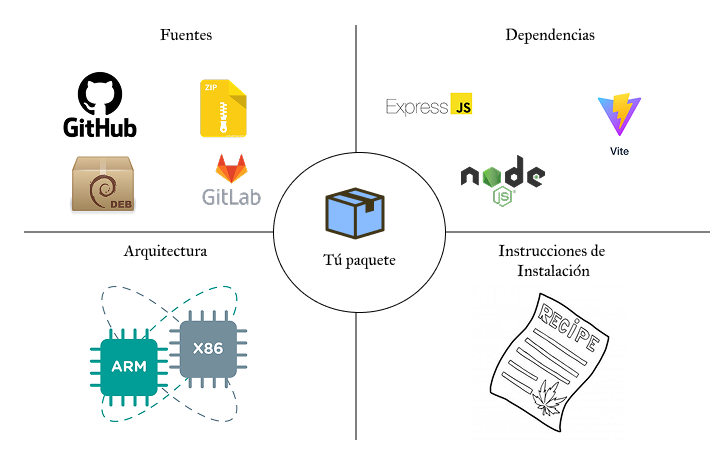
\includegraphics[width=0.5\textwidth]{anexo_diagrama2.png}
\caption{Los diferentes componentes a tomar en cuanta para describir un paquete de \emph{software}}
\label{diagram2}
\end{figure}

\subsubsection{Sección 1 - Manejo de paquetes externos}

Tú manejador de paquetes instala todo dentro de un entorno aislado: cada proyecto tiene su propio espacio con sus propias herramientas, sin interferir con el resto del sistema, similar a un contenedor.

\begin{enumerate}
\item Estas empezando un nuevo proyecto y quieres que todo tu equipo usen las mismas herramientas, tu manejador de paquetes puede hacerlo por ti. Sin embargo, primero tienes que indicar de que fuente obtenerlos. Escribe la sintaxis para indicar que \texttt{fuente1} proviene de \texttt{github.\allowbreak{}com/\allowbreak{}example/\allowbreak{}repo}, \texttt{fuente2} de \texttt{librerias.\allowbreak{}com/\allowbreak{}search} y fuente de un archivo ZIP en \texttt{.\allowbreak{}/\allowbreak{}home/\allowbreak{}user/\allowbreak{}hello}.
\item Antes de indicar que paquetes deseas instalar tienes que indicar para que arquitecturas de computadora debe ser disponible en la sintaxis, sabes que tus compañeros usan \texttt{x86-64-linux} y \texttt{arm64-macos}.
\item Con la configuración previa, escribe la sintaxis para indicar que quieres instalar
\end{enumerate}

\begin{itemize}
\item \texttt{node-v1.0} de \texttt{fuente1}
\item \texttt{reactjs-v2.1} y \texttt{tailwindcss-\allowbreak{}v3.\allowbreak{}0} de \texttt{fuente2}
\item \texttt{vitejs-v1.0} de \texttt{fuente3}.
\end{itemize}

\begin{enumerate}
\setcounter{enumi}{3}
\item Necesitas actualizar \texttt{node} de \texttt{v1.0} a \texttt{v2.0}. Escribe cómo modificarías la declaración anterior.
\item Decidiste que \texttt{vitejs-v1.0} ya no es necesario. Escribe cómo lo eliminarías de la configuración.
\item Un colaborador externo necesita su propio conjunto de herramientas: \texttt{node v2.0} y \texttt{vitest v3.0} pero no quieres reescribir toda la lógica de nuevo para este miembro ¿Cómo escribirías el código para \textbf{reutilizar} lo que ya tienes y definir este  \texttt{ambiente de desarollo}?
\end{enumerate}

\subsubsection{Sección 2 - Manejo de paquetes externos}

Ahora eres tú quien crea un paquete para que otros lo usen. Tienes una aplicación llamada \texttt{mi-app} en \texttt{github.\allowbreak{}com/\allowbreak{}yo/\allowbreak{}mi-\allowbreak{}app} que quieres distribuir.

Construir un paquete ocurre en fases, por ahora trabaja con dos:

\begin{itemize}
\item \textbf{build} --- compilar el código fuente del programa
\item \textbf{install} --- copiar el programa compilado en las carpetas especificas al sistema para que pueda ser usado (\texttt{C:/\allowbreak{}Program Files} en Windows o \texttt{/usr/bin} en Linux).
\end{itemize}

\begin{enumerate}
\item Escribe la sintaxis para declarar este paquete: su nombre, versión \texttt{1.0} de dónde descargarlo y las arquitecturas en donde es soportado.
\item Tu aplicación necesita \texttt{node-v2.0} y \texttt{reactjs-v2.1} para funcionar. Escribe cómo agregarías esas dependencias a la declaración anterior, recuerda que también tienes que indicar de dónde obtenerlas.
\item Escribe la sintaxis para describir la fase \textbf{build} de \texttt{mi-app}: compilar el código ejecutando \texttt{npm run build}.
\item Escribe la sintaxis para describir la fase \textbf{install}: copiar el resultado de la compilación al sistema ejecutando \texttt{npm run install}.
\item Ahora, en \texttt{x86-64-linux} necesitas \texttt{openssl-v1} pero en \texttt{arm64-macos} necesitas \texttt{openssl-v2}. ¿Cómo expresarías que una dependencia cambia según la arquitectura?
\item Como generalizarías tus ideas anteriores para que pudieras definir varios paquetes en un archivo sin tener que repetir tanto código.
\end{enumerate}

\subsection{Guia Entrevistador Pensar en Alto}

\subsubsection{Introducción}

\emph{Leer en voz alta al participante:}

\begin{cajagris}
Gracias por participar. Esta sesión nos ayuda a entender cómo las personas aprenden y razonan con un nuevo lenguaje de programación.

Lo que harás es resolver una serie de pasos para construir un archivo de configuración en Nix. No es un examen --- no hay respuestas correctas o incorrectas, nos interesa tu proceso.

Lo más importante es que hables en voz alta mientras trabajas. Queremos escuchar lo que piensas en cada momento: lo que estás leyendo, lo que esperas que pase, cuando algo no tiene sentido, o cuando crees haber encontrado la solución.

Tu voz y pantalla serán grabadas durante toda la sesión.

¿Tienes alguna pregunta antes de comenzar?
\end{cajagris}

\subsubsection{Recursos disponibles}

\emph{Entregar al participante los siguientes enlaces:}

\begin{itemize}
\item \href{https://nix.dev}{nix.dev}
\item \href{https://search.nixos.org/packages}{search.nixos.org/packages}
\item \href{https://wiki.nixos.org/wiki/Flakes}{wiki.nixos.org/wiki/Flakes}
\item \href{https://noogle.dev}{noogle.dev}
\end{itemize}

\emph{Leer al participante:}

\begin{cajagris}
Puedes consultar estos recursos o buscar en internet libremente. No se permite el uso Inteligencia Artificial como ChatGPT o similares durante la sesión.
\end{cajagris}

\subsubsection{Durante la sesión}

\begin{itemize}
\item No ofrecer pistas ni confirmar si el participante va bien
\item Si el participante guarda silencio por más de 15 segundos, preguntar: \emph{``¿Qué estás pensando ahora?''}
\item Tomar nota de momentos de confusión, bloqueos o sorpresa
\end{itemize}

\subsubsection{Al finalizar}

\begin{itemize}
\item Detener la grabación
\item Agradecer al participante
\item Abrir espacio para preguntas o comentarios
\end{itemize}

\subsubsection{Actividades}

\begin{enumerate}
\item Crear un archivo \texttt{flake.nix} con los campos \texttt{description}, \texttt{inputs} y \texttt{outputs}. Hazlo de tal manera que puedas correr \texttt{nix flake show} sin errores.
\item Agrega \texttt{nixpkgs} como \texttt{input} apuntando a \texttt{github:NixOS/\allowbreak{}nixpkgs/\allowbreak{}release-\allowbreak{}26.\allowbreak{}05}.
\item Has que \texttt{outputs} sea una función que reciba los parámetros \texttt{self} y \texttt{nixpkgs} y retorne un \emph{attribute set} con una llave \texttt{version} y valor \texttt{nixpkgs.\allowbreak{}lib.\allowbreak{}version}. Verifica que corre sin errores con \texttt{nix eval .\allowbreak{}\#version}
\item Modifica tu función \texttt{outputs} para que declaré una variable \texttt{pkgs} que guarde los resultados de importar \texttt{nixpkgs} configurado para \texttt{x84\textunderscore{}64-linux}.
\item Quieres crear un entorno de desarollo (\texttt{devShell}) para la arquitectura \texttt{x84\textunderscore{}64-linux}. Utiliza la función \texttt{pkgs.mkShell} para construirla, basta con que especifiques el atributo \texttt{name}. Entra a ella con el comando \texttt{nix develop}.
\item Agrega aplicaciones \texttt{jp} y \texttt{tree} a tu entorno de desarrollo. Verifica que estan disponibles dentro del entorno.
\item Quisieras que este mismo entorno de desarrollo estuviera disponible para otras arquitecturas, pero no quieres repetir la configuración para cada una. ¿Cómo lo resolverías?
\end{enumerate}

\section{Cuestionarios Fase 2}\label{Appendix4}

\subsection{Cuestionario de comprensión cognitiva de NixLang}

\textbf{Marca en una escala del 1 al 5 tu nivel de experiencia en cada uno de los siguientes temas.}

\emph{Manejo de Paquetes}

\begingroup\renewcommand{\arraystretch}{1.6}
\noindent\begin{tabularx}{\linewidth}{l *{5}{>{\centering\arraybackslash}X} l}
Muy poca & \cuadrito & \cuadrito & \cuadrito & \cuadrito & \cuadrito & Muy avanzada \\
\end{tabularx}
\endgroup

\emph{TypeScript}

\begingroup\renewcommand{\arraystretch}{1.6}
\noindent\begin{tabularx}{\linewidth}{l *{5}{>{\centering\arraybackslash}X} l}
Muy poca & \cuadrito & \cuadrito & \cuadrito & \cuadrito & \cuadrito & Muy avanzada \\
\end{tabularx}
\endgroup

\emph{NixLang}

\begingroup\renewcommand{\arraystretch}{1.6}
\noindent\begin{tabularx}{\linewidth}{l *{5}{>{\centering\arraybackslash}X} l}
Muy poca & \cuadrito & \cuadrito & \cuadrito & \cuadrito & \cuadrito & Muy avanzada \\
\end{tabularx}
\endgroup

\emph{Lenguajes Funcionales}

\begingroup\renewcommand{\arraystretch}{1.6}
\noindent\begin{tabularx}{\linewidth}{l *{5}{>{\centering\arraybackslash}X} l}
Muy poca & \cuadrito & \cuadrito & \cuadrito & \cuadrito & \cuadrito & Muy avanzada \\
\end{tabularx}
\endgroup

\subsubsection{Instrucciones}

Se te presentaran una serie de ejercicios para poner a prueba tu aprendizaje en \textbf{NixLang}.

Durante la prueba puedes consultar el contenido de aprendizaje dado por el investigador, como buscar por internet, más \textbf{no se permite el uso de asistentes de inteligencia artificial}.

\textbf{PA1-1}. Escoge el código correcto (Sin errores sintácticos).

\begin{opcion}{a)}
\begin{lstlisting}[language=nix]
{
  description = "A simple development environment"
  inputs.nixpkgs.url = "github:NixOS/nixpkgs/nixos-unstable";
  outputs = { self, nixpkgs }:
    let
      system = "x86_64-linux";
      pkgs = nixpkgs.legacyPackages.${system};
    in {
      devShells.${system}.default = pkgs.mkShell {
        buildInputs = [ pkgs.python3 pkgs.git ];
        shellHook = ''
          echo "Welcome to the dev shell"
        '';
      };
    };
}
\end{lstlisting}
\end{opcion}

\begin{opcion}{b)}
\begin{lstlisting}[language=nix]
{
  description := "A simple development environment";
  inputs.nixpkgs.url := "github:NixOS/nixpkgs/nixos-unstable";
  outputs = { self, nixpkgs }:
    let
      system := "x86_64-linux";
      pkgs := nixpkgs.legacyPackages.${system};
    in {
      devShells.${system}.default = pkgs.mkShell {
        buildInputs := [ pkgs.python3, pkgs.git ];
        shellHook := "echo Welcome to the dev shell";
      };
    };
}
\end{lstlisting}
\end{opcion}

\begin{opcion}{c)}
\begin{lstlisting}[language=nix]
{
  description = "A simple development environment";
  inputs.nixpkgs.url = "github:NixOS/nixpkgs/nixos-unstable";
  outputs = { self, nixpkgs }:
    let
      system = "x86_64-linux";
      pkgs = nixpkgs.legacyPackages.$(system);
    in {
      devShells.$(system).default = pkgs.mkShell {
        buildInputs = [ pkgs.python3 pkgs.git ];
        shellHook = ''
          echo "Welcome to the dev shell"
        '';
      };
    };
}
\end{lstlisting}
\end{opcion}

\begin{opcion}{d)}
CORRECTA
\begin{lstlisting}[language=nix]
{
  description = "A simple development environment";
  inputs.nixpkgs.url = "github:NixOS/nixpkgs/nixos-unstable";
  outputs = { self, nixpkgs }:
    let
      system = "x86_64-linux";
      pkgs = nixpkgs.legacyPackages.${system};
    in {
      devShells.${system}.default = pkgs.mkShell {
        buildInputs = [ pkgs.python3 pkgs.git ];
        shellHook = ''
          echo "Welcome to the dev shell"
        '';
      };
    };
}
\end{lstlisting}
\end{opcion}

\begin{opcion}{e)}
\begin{lstlisting}[language=nix]
{
  description = "A simple development environment";
  inputs.nixpkgs.url = "github:NixOS/nixpkgs/nixos-unstable";
  outputs = { self, nixpkgs }:
    let
      system = "x86_64-linux";
      pkgs = nixpkgs.legacyPackages.${system}
    in {
      devShells.${system}.default = pkgs.mkShell {
        buildInputs = [ pkgs.python3 pkgs.git];
        shellHook = ''
          echo "Welcome to the dev shell"
        '';
      };
    };
}
\end{lstlisting}
\end{opcion}

\textbf{PA1-2}. \emph{(Opcional)} Escoge el código correcto (Sin errores sintácticos).

\begin{opcion}{a)}
\begin{lstlisting}[language=nix]
# more code...
packages.${system}.default = pkgs.stdenv.mkDerivation {
  pname = "greet"
  version = "1.0.0";
  src = pkgs.fetchFromGitHub {
    owner = "example";
    repo = "greet";
    rev = "v1.0.0";
    sha256 = "AAAA...";
  };
  buildPhase = ''
    gcc -O2 -o greet main.c
  '';
  installPhase = ''
    mkdir -p $out/bin
    cp greet $out/bin/greet
  '';
};
# more code...
\end{lstlisting}
\end{opcion}

\begin{opcion}{b)}
CORRECTA
\begin{lstlisting}[language=nix]
# more code...
packages.${system}.default = pkgs.stdenv.mkDerivation {
  pname = "greet";
  version = "1.0.0";
  src = pkgs.fetchFromGitHub {
    owner = "example";
    repo = "greet";
    rev = "v1.0.0";
    sha256 = "AAAA...";
  };
  nativeBuildInputs = [ pkgs.gcc ];
  buildPhase = ''
    gcc -O2 -o greet main.c
  '';
  installPhase = ''
    mkdir -p $out/bin
    cp greet $out/bin/greet
  '';
};
# more code...
\end{lstlisting}
\end{opcion}

\begin{opcion}{c)}
\begin{lstlisting}[language=nix]
# more code...
packages.${system}.default := pkgs.stdenv.mkDerivation {
  pname := "greet";
  version := "1.0.0";
  src := pkgs.fetchFromGitHub(
    owner: "example",
    repo: "greet",
    rev: "v1.0.0",
    sha256: "AAAA...");
  buildPhase := "gcc -O2 -o greet main.c";
  installPhase := "mkdir -p $out/bin; cp greet $out/bin/greet";
};
# more code...
\end{lstlisting}
\end{opcion}

\begin{opcion}{d)}
\begin{lstlisting}[language=nix]
# more code...
packages.${system}.default = pkgs.stdenv.mkDerivation {
  pname = "greet";
  version = "1.0.0"
  src = pkgs.fetchFromGitHub {
    owner: "example";
    repo: "greet";
    rev: "v1.0.0";
    sha256: "AAAA...";
  }
  buildPhase = ''
    gcc -O2 -o greet main.c
  '';
  installPhase = ''
    mkdir -p $out/bin
    cp greet $out/bin/greet
  '';
};
# more code...
\end{lstlisting}
\end{opcion}

\begin{opcion}{e)}
\begin{lstlisting}[language=nix]
# more code...
packages.${system}.default = pkgs.stdenv.mkDerivation {
  pname = "greet";
  version = "1.0.0";
  src = pkgs.fetchFromGitHub {
    owner = "example",
    repo = "greet",
    rev = "v1.0.0",
    sha256 = "AAAA...",
  };
  buildPhase = ''
    gcc -O2 -o greet main.c
  '';
  installPhase = ''
    mkdir -p $out/bin
    cp greet $out/bin/greet
  '';
};
# more code...
\end{lstlisting}
\end{opcion}

\textbf{PA2-1}. Selecciona el trozo de código que \textbf{NO} tiene sentido.

\begin{opcion}{a)}
\begin{lstlisting}[language=nix]
#  ...
devShells.${system}.default = pkgs.mkShell {
  buildInputs = [ pkgs.python3 ];
  shellHook = ''
    echo "Welcome to the dev shell"
  '';
};
#  ...
\end{lstlisting}
\end{opcion}

\begin{opcion}{b)}
\begin{lstlisting}[language=nix]
#  ...
devShells.${system}.default = pkgs.mkShell {
  buildInputs = [ pkgs.python3 pkgs.git ];
  shellHook = builtins.concatStringsSep " " [ "echo" "Welcome to the dev shell" ];
};
#  ...
\end{lstlisting}
\end{opcion}

\begin{opcion}{c)}
CORRECTA
\begin{lstlisting}[language=nix]
#  ...
system = pkgs.git;
pkgs = nixpkgs.legacyPackages.${system};
devShells.${system}.default = pkgs.mkShell {
  buildInputs = [ pkgs.python3 pkgs.git ];
};
#  ...
\end{lstlisting}
\end{opcion}

\begin{opcion}{d)}
\begin{lstlisting}[language=nix]
#  ...
devShells.${system}.default = pkgs.mkShell {
  buildInputs = [ pkgs.python3 pkgs.git pkgs.nodejs ];
  shellHook = ''
    echo "Welcome to the dev shell"
  '';
};
#  ...
\end{lstlisting}
\end{opcion}

\begin{opcion}{e)}
\begin{lstlisting}[language=nix]
#  ...
devShells.${system}.default = pkgs.mkShell {
  buildInputs = [ pkgs.python3 pkgs.git ];
  shellHook = ''
    echo "Welcome to the dev shell"
  '';
};
#  ...
\end{lstlisting}
\end{opcion}

\textbf{PA2-2}. \emph{(Opcional)} Selecciona el trozo de código que \textbf{SI} tiene sentido.

\begin{opcion}{a)}
CORRECTA
\begin{lstlisting}[language=nix]
#  ...
pkgs.stdenv.mkDerivation{
  pname = "greet";
  version = "1.0.0";
  src = pkgs.fetchFromGitHub { owner = "example"; repo = "greet"; rev = "v1.0.0"; sha256 = "AAAA..."; };
  nativeBuildInputs = with pkgs; [gcc];
  buildPhase = ''gcc -O2 -o greet main.c'';
  installPhase = ''mkdir -p $out/bin; cp greet $out/bin/greet'';
}
#  ...
\end{lstlisting}
\end{opcion}

\begin{opcion}{b)}
\begin{lstlisting}[language=nix]
#  ...
pkgs.stdenv.mkDerivation {
  pname = "greet";
  version = "1.0.0";
  src = pkgs.fetchFromGitHub { owner = "example"; repo = "greet"; rev = "v1.0.0"; sha256 = "AAAA..."; };
  nativeBuildInputs = pkgs.gcc;
  buildPhase = ''gcc -O2 -o greet main.c'';
  installPhase = ''mkdir -p $out/bin; cp greet $out/bin/greet'';
}
#  ...
\end{lstlisting}
\end{opcion}

\begin{opcion}{c)}
\begin{lstlisting}[language=nix]
#  ...
pkgs.stdenv.mkDerivation {
  pname = "greet";
  version = "1.0.0";
  src = pkgs.fetchFromGitHub { owner = "example"; repo = "greet"; rev = "v1.0.0"; sha256 = "AAAA..."; };
  nativeBuildInputs = [ pkgs.gcc ];
  buildPhase = ''gcc -O2 -o greet main.c'';
  installPhase = $out;
}
#  ...
\end{lstlisting}
\end{opcion}

\begin{opcion}{d)}
\begin{lstlisting}[language=nix]
#  ...
pkgs.stdenv.mkDerivation {
  pname = "greet";
  version = "1.0.0";
  src = "main.c";
  nativeBuildInputs = [ pkgs.gcc ];
  buildPhase = ''gcc -O2 -o greet main.c'';
  installPhase = ''mkdir -p $out/bin; cp greet $out/bin/greet'';
}
#  ...
\end{lstlisting}
\end{opcion}

\begin{opcion}{e)}
\begin{lstlisting}[language=nix]
#  ...
pkgs.stdenv.mkDerivation {
  pname = "greet";
  version = "1.0.0";
  src = pkgs.fetchFromGitHub {
    owner = "example";
    repo = "greet";
    rev = "v1.0.0";
    sha256 = "AAAA..."; };
  buildPhase = ''gcc -O2 -o greet main.c'';
  installPhase = ''mkdir -p $out/bin; cp greet $out/bin/greet'';
  buildPhase = ''make'';
}
#  ...
\end{lstlisting}
\end{opcion}

\textbf{PA3-1}. Selecciona el programa correcto con el resultado solicitado.

\emph{``Dado \texttt{x = 10}, seleciona el programa que evalúa correctamente a `grande'.''}

\begin{opcion}{a)}
CORRECTA
\begin{lstlisting}[language=nix]
let
  x = 10;
in
if x < 5 then "pequeño"
else if x < 10 then "mediano"
else "grande"
\end{lstlisting}
\end{opcion}

\begin{opcion}{b)}
\begin{lstlisting}[language=nix]
let
  x = 10;
in
if x < 5 then "pequeño"
else if x <= 10 then "mediano"
else "grande"
\end{lstlisting}
\end{opcion}

\begin{opcion}{c)}
\begin{lstlisting}[language=nix]
let
  x = 10;
in
if x > 10 then "grande"
else if x > 5 then "mediano"
else "pequeño"
\end{lstlisting}
\end{opcion}

\begin{opcion}{d)}
\begin{lstlisting}[language=nix]
let
  x = 10;
in
if x < 5 then "manzanas"
else if x < 10 then "peras"
else "bananos"
\end{lstlisting}
\end{opcion}

\begin{opcion}{e)}
\begin{lstlisting}[language=nix]
let
  x = 10;
in
if x < 5 then "pequeño"
else if x < 10 then "mediano"
\end{lstlisting}
\end{opcion}

\textbf{PA3-2}. \emph{(Opcional)} Selecciona el programa correcto con el resultado solicitado.

\emph{``Un programa de nixlang que produzca una \textbf{DevShell} para linux 🐧, y construya un paquete para macos 🍎 (Darwin).''}

\begin{opcion}{a)}
\begin{lstlisting}[language=nix]
out = {} : let
  pkgsLinux = import nixpkgs { system = "x86_64-linux"; };
  pkgsMacos = import nixpkgs { system = "x86_64-darwin"; };
in {
  devShells.x86_64-linux.default = pkgsMacos.stdenv.mkDerivation {
    #... more code
  };
  packages.x86_64-darwin.default = pkgsLinux.stdenv.mkDerivation {
    #... more code
  };
};
\end{lstlisting}
\end{opcion}

\begin{opcion}{b)}
\begin{lstlisting}[language=nix]
{
  outputs = { self, nixpkgs }:
    let
      pkgs = import nixpkgs { system = "x86_64-linux"; };
    in {
      devShells.default = pkgs.mkShell {
        #... more code
      };
      packages.default = pkgs.stdenv.mkDerivation {
        #... more code
      };
    };
}
\end{lstlisting}
\end{opcion}

\begin{opcion}{c)}
CORRECTA
\begin{lstlisting}[language=nix]
{
  outputs = { self, nixpkgs }:
    let
      pkgsLinux = import nixpkgs { system = "x86_64-linux"; };
      pkgsMacos = import nixpkgs { system = "x86_64-darwin"; };
    in {
      devShells.x86_64-linux.default = pkgsLinux.mkShell {
        #... more code
      };
      packages.x86_64-darwin.default = pkgsMacos.stdenv.mkDerivation {
        #... more code
      };
    };
}
\end{lstlisting}
\end{opcion}

\begin{opcion}{d)}
\begin{lstlisting}[language=nix]
{
  outputs = { self, nixpkgs }:
    let
      pkgs = import nixpkgs { system = "x86_64-linux"; };
    in {
      devShells.x86_64-linux.default = pkgs.mkShell {
        #... more code
      };
      packages.x86_64-linux.default = pkgs.stdenv.mkDerivation {
        #... more code
      };
    };
}
\end{lstlisting}
\end{opcion}

\begin{opcion}{e)}
\begin{lstlisting}[language=nix]
{
  outputs = { self, nixpkgs }:
    let
      pkgsLinux = import nixpkgs { system = "x86_64-linux"; };
      pkgsMacos = import nixpkgs { system = "x86_64-darwin"; };
    in {
      packages.x86_64-darwin.default = pkgsMacos.stdenv.mkDerivation {
        #... more code
      };
    };
}
\end{lstlisting}
\end{opcion}

\textbf{PP4-1}. Selecciona el valor final de \texttt{[ f a ]} tras ser evaluado.

\begin{bloquecodigo}
\begin{lstlisting}[language=nix]
let
  f = x: x + 1;
  a = 1;
in [ f a ]
\end{lstlisting}
\end{bloquecodigo}

\textbf{a)} \texttt{[ <lambda> 1 ]} (CORRECTA)\\
\textbf{b)} \texttt{[ 2 ]}\\
\textbf{c)} \texttt{2}\\
\textbf{d)} \texttt{[ <lambda> ]}\\
\textbf{e)} Error de evaluación

\textbf{PP4-2}. \emph{(Opcional)} Selecciona el resultado correcto para cuando se corre \texttt{nix build .\allowbreak{}\#default} con el programa dado:

\begin{bloquecodigo}
\begin{lstlisting}[language=nix]
packages.${system}.default = pkgs.stdenv.mkDerivation {
  pname = "greet";
  version = "1.0.0";
  src = pkgs.fetchFromGitHub {
    owner = "example"; repo = "greet"; rev = "v1.0.0"; sha256 = "AAAA...";
  };
  nativeBuildInputs = [ pkgs.gcc ];
  buildPhase = ''gcc -O2 -o greet main.c'';
  installPhase = ''
    mkdir -p $out/bin
    cp greet $out/bin/greet
  '';
};
\end{lstlisting}
\end{bloquecodigo}

\textbf{a)} Nix compila usando el código fuente del directorio de trabajo actual en lugar de GitHub, ya que \texttt{fetchFromGitHub} solo se usa con fines de documentación.\\
\textbf{b)} Nix obtiene el código fuente de GitHub en la revisión fijada, lo verifica con el hash sha256 proporcionado, compila main.c con gcc y genera \texttt{bin/greet}. (CORRECTA)\\
\textbf{c)} Nix crea un entorno de desarrollo (dev shell) con \texttt{gcc} disponible.\\
\textbf{d)} Nix obtiene el código fuente, pero omite la verificación del hash porque sha256 es un valor de marcador de posición, y se ejecuta correctamente sin mostrar ningún error.\\
\textbf{e)} Nix compila el programa correctamente, pero el binario resultante se llama main, no greet, porque ese es el nombre del archivo fuente (\texttt{main.c}).

\textbf{PP5-1}. Identifica cuantas variables son accesibles desde el bloque señalado en el comentario:

\begin{bloquecodigo}
\begin{lstlisting}[language=nix]
{

  description = { };

  inputs = {
    nixpkgs.url = "";
    myconfigs.url = "";
  };

  outputs = { self, nixpkgs, myconfigs }:
    let
      a = "A";
    in
    let
      b = "B";
      c = "C";
    in
    {
      a = let d = "D"; in d;
      b = let
          e = "E";
        in
        {
          # <= HERE
        };
    };
}
\end{lstlisting}
\end{bloquecodigo}

\textbf{a)} 6\\
\textbf{b)} 7 (CORRECTA)\\
\textbf{c)} 8\\
\textbf{d)} 5\\
\textbf{e)} 4

\textbf{PP5-2}. \emph{(Opcional)} En base a la estructura del siguiente código que puedes decir de los tipos de \texttt{x, y, z, a}:

\begin{bloquecodigo}
\begin{lstlisting}[language=nix]
{ x, y, z }: (x y).a z;
\end{lstlisting}
\end{bloquecodigo}

\textbf{a)} \texttt{x} es una función | \texttt{y} es un tipo cualquiera | \texttt{z} es un \emph{attribute set} | \texttt{a} es una función.\\
\textbf{b)} \texttt{x} es una función | \texttt{y} es un tipo cualquiera | \texttt{z} es un tipo cualquiera | \texttt{a} es una función. (CORRECTA)\\
\textbf{c)} \texttt{x} es un \emph{attribute set} | \texttt{y} es una función | \texttt{z} es un tipo cualquiera | \texttt{a} es un tipo cualquiera.\\
\textbf{d)} \texttt{x} es una función | \texttt{y} es un \emph{attribute set} | \texttt{z} es un tipo cualquiera | \texttt{a} es una función.\\
\textbf{e)} \texttt{x} es una función | \texttt{y} es un tipo cualquiera | \texttt{z} es un tipo cualquiera | \texttt{a} es un \emph{attribute set}.

\textbf{PP6-1}. Selecciona el programa que evalué una expresión equivalente a:

\begin{bloquecodigo}
\begin{lstlisting}[language=nix]
{
  pname = "hello";
  version = "0.1";
  meta = {
    mantainers = [ ["1" "1"] ["2" "2"] ];
    source = {
      type = "github";
      remote = "github.com/example/repo";
    };
  };
}
\end{lstlisting}
\end{bloquecodigo}

\begin{opcion}{a)}
\begin{lstlisting}[language=nix]
{
  pname = "hello";
  version = "0.1";
  meta = {
    mantainers = [ ["1" "1"] ["2" "2"] ];
  };
  meta.source.type = "github";
}
\end{lstlisting}
\end{opcion}

\begin{opcion}{b)}
\begin{lstlisting}[language=nix]
let
  data = {
    mantainers = [ ["1" "1"] ["2" "2"] ];
    source = {
      type = "github";
      remote = "github.com/example/repo";
    };
  };
in  {
  pname = "hello";
  version = "0.1";
  meta = { inherit data; };
}
\end{lstlisting}
\end{opcion}

\begin{opcion}{c)}
CORRECTA
\begin{lstlisting}[language=nix]
let
  info = {
    type = "github";
    remote = "github.com/example/repo";
  };
in {
  pname = "hello";
  version = "0.1";
  meta.mantainers = [ ["1" "1"] ["2" "2"] ];
  meta.source = {inherit (info) type remote; };
}
\end{lstlisting}
\end{opcion}

\begin{opcion}{d)}
\begin{lstlisting}[language=nix]
{
  pname = "hello";
  version = "0.1";
  meta = {
    mantainers = [ ["1" "1"] ["2" "2"] ];
    source = {
      type = /github;
      remote = ./github.com/example/repo;
    };
  };
}
\end{lstlisting}
\end{opcion}

\begin{opcion}{e)}
\begin{lstlisting}[language=nix]
{
  pname = "hello";
  version = "0.1";
  meta.mantainers = let
    _a = "1";
    _b = "2";
  in [ _a _a _b _b ] ;
  meta.source = {
    type = "github";
    remote = "github.com/example/repo";
  };
}
\end{lstlisting}
\end{opcion}

\textbf{PP6-2}. \emph{(Opcional)} Selecciona el programa que evalúa a una expresión equivalente a:

\begin{bloquecodigo}
\begin{lstlisting}[language=nix]
{ x = "PKGS-A"; y = "OVERRIDE-B"; z = "OVERRIDE-C"; }
\end{lstlisting}
\end{bloquecodigo}

\begin{opcion}{a)}
\begin{lstlisting}[language=nix]
let
  pkgs = { a = "PKGS-A"; b = "PKGS-B"; };
  overrides = { b = "OVERRIDE-B"; c = "OVERRIDE-C"; };
in
with overrides;
with pkgs;
{
  x = a;
  y = b;
  z = c;
}
\end{lstlisting}
\end{opcion}

\begin{opcion}{b)}
CORRECTA
\begin{lstlisting}[language=nix]
let
  pkgs = { a = "PKGS-A"; b = "PKGS-B"; };
  overrides = { b = "OVERRIDE-B"; c = "OVERRIDE-C"; };
in
with pkgs;
with overrides;
{
  x = a;
  y = b;
  z = c;
}
\end{lstlisting}
\end{opcion}

\begin{opcion}{c)}
\begin{lstlisting}[language=nix]
let
  pkgs = { a = "PKGS-A"; b = "PKGS-B"; };
  overrides = { b = "OVERRIDE-B"; c = "OVERRIDE-C"; };
in
with pkgs;
with overrides;
{
  x = a;
  y = a;
  z = a;
}
\end{lstlisting}
\end{opcion}

\begin{opcion}{d)}
\begin{lstlisting}[language=nix]
let
  pkgs = { a = "PKGS-A"; b = "PKGS-B"; };
  overrides = { b = "OVERRIDE-B"; c = "OVERRIDE-C"; };
in
with overrides // pkgs;
{
  x = a;
  y = b;
  z = c;
}
\end{lstlisting}
\end{opcion}

\begin{opcion}{e)}
\begin{lstlisting}[language=nix]
let
  base = { a = "PKGS-A"; b = "PKGS-B"; };
  patch = { b = "PKGS-A"; c = "PKGS-B"; };
in
with base;
with patch;
{
  x = a;
  y = b;
  z = c;
}
\end{lstlisting}
\end{opcion}

\textbf{PP7-1}. En qué orden crees que se van a evaluar los diferentes atributos de esta expresión, \textbf{recuerda que NixLang evalúa perezosamente}.

El \texttt{\&} significa que se evaluan a la vez en el mismo paso.

\begin{bloquecodigo}
\begin{lstlisting}[language=nix]
let
  content = rec {
    a = 1;
    b = a + 2;
    c = b * 3;
  };
in
content.c # La evaluación empieza aquí.
\end{lstlisting}
\end{bloquecodigo}

\textbf{a)} c $\rightarrow$ b $\rightarrow$ a (CORRECTA)\\
\textbf{b)} a $\rightarrow$ b $\rightarrow$ c\\
\textbf{c)} c \& b $\rightarrow$ a\\
\textbf{d)} a \& b \& c\\
\textbf{e)} c \& a $\rightarrow$ b

\textbf{PP7-2}. \emph{(Opcional)} Indica cual será el resultado de evaluar la siguiente expresión, \textbf{recuerda que NixLang evalúa perezosamente}.

\begin{bloquecodigo}
\begin{lstlisting}[language=nix]
let
  list = [ (1 / 0) (2 / 0) ];
  # Esta operación toma mucho tiempo
  x = builtins.foldl' builtins.add 0 (builtins.genList (i: i) 1000000000000);
in
  if builtins.length list == 2
    then "it's all good!"
    else x
\end{lstlisting}
\end{bloquecodigo}

\textbf{a)} Evalúa a \texttt{"it\textquotesingle{}s all good!"}. (CORRECTA)\\
\textbf{b)} Falla por división por cero.\\
\textbf{c)} Falla por variable indefinida.\\
\textbf{d)} Evalúa a \texttt{"it\textquotesingle{}s all good!"}, pero porque NixLang elimina automáticamente la rama else no usada.\\
\textbf{e)} Tarda mucho en responder, porque NixLang calcula \texttt{x}.

\textbf{PP8-1}. Indica cual será el resultado de la siguiente operación.

\begin{bloquecodigo}
\begin{lstlisting}[language=nix]
let
  numbers = [ 1 2 3 ];
  labels = [
    { name = "a"; value = 1; }
    { name = "b"; value = 2; }
  ];
in
{
  # map aplica una función a cada elemento de una lista,
  # devolviendo una nueva lista con los resultados
  a = map (n: n * 2) numbers;

  # listToAttrs convierte una lista de { name = ...; value = ...; }
  # en un attribute set, usando `name` como clave y `value` como valor
  b = builtins.listToAttrs labels;
}
\end{lstlisting}
\end{bloquecodigo}

\begin{opcion}{a)}
\begin{lstlisting}[language=nix]
{
  a = [ 1 2 3 ];
  b = [ { name = "a"; value = 1; } { name = "b"; value = 2; } ];
}
\end{lstlisting}
\end{opcion}

\begin{opcion}{b)}
\begin{lstlisting}[language=nix]
{
  a = [ 2 4 6 ];
  b = [ 1 2 ];
}
\end{lstlisting}
\end{opcion}

\begin{opcion}{c)}
\begin{lstlisting}[language=nix]
{
  a = 6;
  b = { a = 1; b = 2; };
}
\end{lstlisting}
\end{opcion}

\begin{opcion}{d)}
CORRECTA
\begin{lstlisting}[language=nix]
{
  a = [ 2 4 6 ];
  b = { a = 1; b = 2; };
}
\end{lstlisting}
\end{opcion}

\begin{opcion}{e)}
\begin{lstlisting}[language=nix]
{
  a = [ 2 4 6 ];
  b = { name = "b"; value = 2; };
}
\end{lstlisting}
\end{opcion}

\textbf{PP8-2}. \emph{(Opcional)} Indica cual será el resultado de la siguiente operación. Recuerda que:

\begin{itemize}
\item \texttt{map}: aplica una función a cada elemento de una lista, devolviendo una nueva lista con los resultados
\item \texttt{listToAttrs}: convierte una lista de \texttt{\{ name = .\allowbreak{}.\allowbreak{}.\allowbreak{}; value = .\allowbreak{}.\allowbreak{}.\allowbreak{}; \}} en un attribute set, usando \texttt{name} como clave y \texttt{value} como valor
\end{itemize}

\begin{bloquecodigo}
\begin{lstlisting}[language=nix]
let
  inventoryCreator =
    items: # Lista de nombres de items.
    # El resultado de map es dado a la funcion listToAttrs.
    (builtins.listToAttrs (
      map (item: {
        name = item; # Nombre del elemento;
        value = 100; # Cantidad de dicho item;
      }) items
    ));
in
inventoryCreator [ "banana" "apple" ]
\end{lstlisting}
\end{bloquecodigo}

\begin{opcion}{a)}
\begin{lstlisting}[language=nix]
error: attribute 'value' missing
\end{lstlisting}
\end{opcion}

\begin{opcion}{b)}
CORRECTA
\begin{lstlisting}[language=nix]
{ banana = 100; apple = 100; }
\end{lstlisting}
\end{opcion}

\begin{opcion}{c)}
\begin{lstlisting}[language=nix]
[
  { name = "banana"; value = 100; }
  { name = "apple"; value = 100; }
]
\end{lstlisting}
\end{opcion}

\begin{opcion}{d)}
\begin{lstlisting}[language=nix]
{ banana = null; apple = null; }
\end{lstlisting}
\end{opcion}

\begin{opcion}{e)}
\begin{lstlisting}[language=nix]
{ name = "apple"; value = 100; }
\end{lstlisting}
\end{opcion}

\subsubsection{Respuestas Libres}

\textbf{En esta sección editaras \texttt{weathercli} un programa ya empaquetado con Nix}. En cada ejercicio deberás modificar el código siguiendo las instrucciones.

\textbf{Se te proporcionará un entorno de desarrollo en línea (Codespaces)} con todas las herramientas necesarias, por lo que no necesitas instalar nada en tu computadora.

Abre ahora el entorno: \href{https://codespaces.new/DanielRasho/Thesis-codespaces?quickstart=1&devcontainer_path=.devcontainer/nix/devcontainer.json}{\underline{Abrir Codespace}}\footnote{\url{https://codespaces.new/DanielRasho/Thesis-codespaces?quickstart=1&devcontainer_path=.devcontainer/nix/devcontainer.json}}. Tarda unos minutos en iniciar; déjalo abierto en otra pestaña.

Para cada ejercicio:

\begin{enumerate}
\item Lee la instrucción.
\item Modifica el código proporcionado.
\item Guarda el archivo (\texttt{Ctrl+S}) y verifica que la solución funcione desde una terminal del Codespace (menú \emph{Terminal $\rightarrow$ New Terminal}). \textbf{Cada ejercicio indica qué comando usar y qué resultado esperar}.
\item Cuando estés conforme con tu respuesta, copia el código solicitado y pégalo en el cuestionario.
\item No cierres el editor, lo usarás en cada ejercicio.
\end{enumerate}

\textbf{Los ejercicios son independientes entre sí. Si no logras resolver uno, puedes continuar con el siguiente.}

\textbf{PE9-1}. Abre \textbf{Codespaces} (link abajo), trabajaras en \texttt{flake.nix}. Reemplaza el contenido con el \textbf{Código inicial}.

\textbf{Contexto}\\
Has empaquetado \textbf{\texttt{weathercli}} un script que consulta el clima de una ciudad. Actualmente el paquete solo está disponible para la plataforma \texttt{x86\textunderscore{}64-linux}.

\textbf{Instrucciones}\\
Modifica el archivo \texttt{flake.nix} para que también soporte los siguientes sistemas:

\begin{itemize}
\item \texttt{x86\textunderscore{}64-linux}
\item \texttt{aarch64-linux}
\item \texttt{x86\textunderscore{}64-darwin}
\item \texttt{aarch64-darwin}
\end{itemize}

\textbf{Cómo probarlo}\\
Ejecuta \texttt{nix flake show}. Bajo \texttt{packages} deben aparecer los 4 sistemas (los que no son el del Codespace aparecen como \texttt{omitted}, eso es normal):

\begin{bloquecodigo}
\begin{lstlisting}
└───packages
    ├───aarch64-darwin
    │   └───weathercli omitted (use '--all-systems' to show)
    ├───aarch64-linux
    │   └───weathercli omitted (use '--all-systems' to show)
    ├───x86_64-darwin
    │   └───weathercli omitted (use '--all-systems' to show)
    └───x86_64-linux
        └───weathercli: package 'weathercli-1.0.0'
\end{lstlisting}
\end{bloquecodigo}

Luego ejecuta \texttt{nix run .\allowbreak{}\#weathercli}: el programa debe seguir funcionando y mostrar el clima de Tokyo:

\begin{bloquecodigo}
\begin{lstlisting}
https://wttr.in/Tokyo?m&format=%l:+%c+%t
Tokyo: ☀️  +23°C
\end{lstlisting}
\end{bloquecodigo}

Cuando termines, copia todo el contenido de \texttt{flake.nix} y pégalo abajo.

\textbf{❓ Pista}: Puedes definir primero una lista con los sistemas y luego usar \texttt{nixpkgs.\allowbreak{}lib.\allowbreak{}genAttrs} para generar automáticamente los atributos para cada una de ellas.

\href{https://codespaces.new/DanielRasho/Thesis-codespaces?quickstart=1&devcontainer_path=.devcontainer/nix/devcontainer.json}{\underline{Abrir Codespace}}

\textbf{Código inicial}

\begin{bloquecodigo}
\begin{lstlisting}[language=nix]
{
  description = "weathercli — reporte del clima en la terminal";

  inputs.nixpkgs.url = "github:NixOS/nixpkgs/nixos-unstable";

  outputs =
    { self, nixpkgs }:
    {
      # PACKAGES
      # ===========
      packages = {
        x86_64-linux =
        let
          pkgs = nixpkgs.legacyPackages.x86_64-linux;

          defaultConfig = pkgs.writeText "weathercli-config.json" (
            builtins.toJSON {
              city = "Tokyo";
              units = "metric";
              format = "compact";
            }
          );
        in
        {
          # Paquete WeatherCLI
          weathercli = pkgs.stdenv.mkDerivation {
            pname = "weathercli";
            version = "1.0.0";

            src = ./.;

            nativeBuildInputs = [ pkgs.makeWrapper ];

            dontBuild = true;

            installPhase = ''
              mkdir -p $out/bin $out/share/weathercli
              install -m755 weathercli.sh $out/bin/weathercli
              install -m644 ${defaultConfig} $out/share/weathercli/config.json
            '';

            postFixup = ''
              wrapProgram $out/bin/weathercli \
                --prefix PATH : ${
                  pkgs.lib.makeBinPath [
                    pkgs.curl
                    pkgs.jq
                  ]
                } \
                --set-default WEATHERCLI_CONFIG "$out/share/weathercli/config.json"
            '';
          };
        };
      };
    };
}
\end{lstlisting}
\end{bloquecodigo}

\textbf{PE10-1}. \textbf{Antes de empezar, reemplaza todo el contenido de \texttt{flake.nix} con el código inicial de abajo.}

\textbf{Contexto}\\
\texttt{weathercli} utiliza un archivo de configuración llamado \texttt{weathercli-\allowbreak{}config.\allowbreak{}json} para indicar la ciudad a consultar. Sin embargo, el programa \textbf{también funciona si ese archivo no existe}.

Actualmente ese archivo es creado por Nix.

\textbf{Instrucciones}\\
Modifica el código para que Nix deje de generar el archivo de configuración.

\textbf{Cómo probarlo}\\
Ejecuta \texttt{nix run ".\allowbreak{}\#weathercli"}. Debería mostrar una ciudad diferente a Roma:

\begin{bloquecodigo}
\begin{lstlisting}
https://wttr.in/?m&format=%l:+%c+%t
Ashburn, Virginia, US: ☀️  +18°C
\end{lstlisting}
\end{bloquecodigo}

Cuando termines, copia todo el contenido de \texttt{flake.nix} y pégalo abajo.

\textbf{❓ Pista}: Busca la parte del código donde se crea o escribe el archivo \texttt{weathercli-\allowbreak{}config.\allowbreak{}json} y los lugares donde son usadas.

\href{https://codespaces.new/DanielRasho/Thesis-codespaces?quickstart=1&devcontainer_path=.devcontainer/nix/devcontainer.json}{\underline{Abrir Codespace}}

\textbf{Código inicial}

\begin{bloquecodigo}
\begin{lstlisting}[language=nix]
{
  description = "weathercli — reporte del clima en la terminal";

  inputs.nixpkgs.url = "github:NixOS/nixpkgs/nixos-unstable";

  outputs =
    { self, nixpkgs }:
    let
      systems = [
        "x86_64-linux"
        "aarch64-linux"
        "x86_64-darwin"
        "aarch64-darwin"
      ];
      #  Crea una derivación para cada sistemas
      forAllSystems = nixpkgs.lib.genAttrs systems;
    in
    {
      # PACKAGES
      # ==========
      packages = forAllSystems (
        system:
        let
          pkgs = nixpkgs.legacyPackages.${system};

          # Genera el archivo de configuración por defecto como JSON,
          # a partir de un attribute set de Nix.
          defaultConfig = pkgs.writeText "weathercli-config.json" (
            builtins.toJSON {
              city = "Roma";
              units = "metric";
              format = "compact";
            }
          );
        in
        {
          # Paquete WeatherCLI
          weathercli = pkgs.stdenv.mkDerivation {
            pname = "weathercli";
            version = "1.0.0";
            src = ./.;
            nativeBuildInputs = [ pkgs.makeWrapper ];

            dontBuild = true;

            installPhase = ''
              mkdir -p $out/bin $out/share/weathercli
              install -m755 weathercli.sh $out/bin/weathercli
              install -m644 ${defaultConfig} $out/share/weathercli/config.json
            '';

            postFixup = ''
              wrapProgram $out/bin/weathercli \
                --prefix PATH : ${
                  pkgs.lib.makeBinPath [
                    pkgs.curl
                    pkgs.jq
                  ]
                } \
                --set-default WEATHERCLI_CONFIG "$out/share/weathercli/config.json"
            '';

            meta = {
              description = "Reporte del clima en la terminal, configurable vía un archivo JSON";
              mainProgram = "weathercli";
              platforms = pkgs.lib.platforms.unix;
              license = pkgs.lib.licenses.mit;
            };
          };
        }
      );
    };
}
\end{lstlisting}
\end{bloquecodigo}

\textbf{PE11-1}. \textbf{Antes de empezar, reemplaza todo el contenido de \texttt{flake.nix} con el código inicial de abajo.}

\textbf{Contexto}\\
\texttt{weathercli} ya está correctamente empaquetado. Ahora quieres crear una \texttt{devShell} donde ese paquete esté disponible.

\textbf{Instrucciones}\\
Modifica el código para crear una \texttt{devShell} llamada \texttt{default} (\texttt{devShells.\allowbreak{}<sistema>.\allowbreak{}default}) que incluya el paquete \texttt{weathercli}.

\textbf{Cómo probarlo}\\
Ejecuta \texttt{nix develop} para entrar al entorno y, dentro de él, ejecuta \texttt{weathercli}. Debe mostrar el clima de Roma:

\begin{bloquecodigo}
\begin{lstlisting}
https://wttr.in/Roma?m&format=%l:+%c+%t
Roma: ☀️  +23°C
\end{lstlisting}
\end{bloquecodigo}

Sal del entorno con \texttt{exit}.

Cuando termines, copia todo el contenido de \texttt{flake.nix} y pégalo abajo.

\textbf{❓ Pista:} Puedes acceder al paquete de \texttt{weathercli} mediante el atributo \texttt{self}, por ejemplo: \texttt{self.\allowbreak{}packages.\allowbreak{}x86\textunderscore{}\allowbreak{}64-\allowbreak{}linux.\allowbreak{}weathercli}. Y crear una devShell con \texttt{pkgs.mkShell}.

\href{https://codespaces.new/DanielRasho/Thesis-codespaces?quickstart=1&devcontainer_path=.devcontainer/nix/devcontainer.json}{\underline{Abrir Codespace}}

\textbf{Código inicial}

\begin{bloquecodigo}
\begin{lstlisting}[language=nix]
{
  description = "weathercli — reporte del clima en la terminal";

  inputs.nixpkgs.url = "github:NixOS/nixpkgs/nixos-unstable";

  outputs =
    { self, nixpkgs }:
    let
      systems = [
        "x86_64-linux"
        "aarch64-linux"
        "x86_64-darwin"
        "aarch64-darwin"
      ];
      # Metodo para crear paquetes para cada sistema
      forAllSystems = nixpkgs.lib.genAttrs systems;
    in
    {
      # PACKAGES
      # ===========
      packages = forAllSystems (
        system:
        let
          pkgs = nixpkgs.legacyPackages.${system};

          # Genera el archivo de configuración por defecto como JSON,
          # a partir de un attribute set de Nix.
          defaultConfig = pkgs.writeText "weathercli-config.json" (
            builtins.toJSON {
              city = "Roma";
              units = "metric";
              format = "compact";
            }
          );
        in
        {
          # WeatherCLI package
          weathercli = pkgs.stdenv.mkDerivation {
            pname = "weathercli";
            version = "1.0.0";
            src = ./.;
            nativeBuildInputs = [ pkgs.makeWrapper ];
            dontBuild = true;
            installPhase = ''
              mkdir -p $out/bin $out/share/weathercli
              install -m755 weathercli.sh $out/bin/weathercli
              install -m644 ${defaultConfig} $out/share/weathercli/config.json
            '';
            postFixup = ''
              wrapProgram $out/bin/weathercli \
                --prefix PATH : ${
                  pkgs.lib.makeBinPath [
                    pkgs.curl
                    pkgs.jq
                  ]
                } \
                --set-default WEATHERCLI_CONFIG "$out/share/weathercli/config.json"
            '';
            meta = {
              description = "Reporte del clima en la terminal, configurable vía un archivo JSON";
              mainProgram = "weathercli";
              platforms = pkgs.lib.platforms.unix;
              license = pkgs.lib.licenses.mit;
            };
          };
        }
      );
      # DEVSHELLS
      # ===========
      # escribe aqui...
    };
}
\end{lstlisting}
\end{bloquecodigo}

\subsection{Cuestionario de comprensión cognitiva de Nixty}

\textbf{Marca en una escala del 1 al 5 tu nivel de experiencia en cada uno de los siguientes temas.}

\emph{Manejo de Paquetes}

\begingroup\renewcommand{\arraystretch}{1.6}
\noindent\begin{tabularx}{\linewidth}{l *{5}{>{\centering\arraybackslash}X} l}
Muy poca & \cuadrito & \cuadrito & \cuadrito & \cuadrito & \cuadrito & Muy avanzada \\
\end{tabularx}
\endgroup

\emph{TypeScript}

\begingroup\renewcommand{\arraystretch}{1.6}
\noindent\begin{tabularx}{\linewidth}{l *{5}{>{\centering\arraybackslash}X} l}
Muy poca & \cuadrito & \cuadrito & \cuadrito & \cuadrito & \cuadrito & Muy avanzada \\
\end{tabularx}
\endgroup

\emph{NixLang}

\begingroup\renewcommand{\arraystretch}{1.6}
\noindent\begin{tabularx}{\linewidth}{l *{5}{>{\centering\arraybackslash}X} l}
Muy poca & \cuadrito & \cuadrito & \cuadrito & \cuadrito & \cuadrito & Muy avanzada \\
\end{tabularx}
\endgroup

\emph{Lenguajes Funcionales}

\begingroup\renewcommand{\arraystretch}{1.6}
\noindent\begin{tabularx}{\linewidth}{l *{5}{>{\centering\arraybackslash}X} l}
Muy poca & \cuadrito & \cuadrito & \cuadrito & \cuadrito & \cuadrito & Muy avanzada \\
\end{tabularx}
\endgroup

\subsubsection{Instrucciones}

Se te presentaran una serie de ejercicios para poner a prueba tu aprendizaje en \textbf{Nixty}.

Durante la prueba puedes consultar el contenido de aprendizaje dado por el investigador, como buscar por internet, más \textbf{no se permite el uso de asistentes de inteligencia artificial}.

\textbf{PA1-1}. Escoge el código correcto (Sin errores sintácticos).

\begin{opcion}{a)}
\begin{lstlisting}[language=TypeScript]
import { Definition, DevShell, Nixpkgs, System } from "nixty-lib"

const NIX_PKGS = new Nixpkgs({ tag: "nixos-unstable" })

const dev = new DevShell({
    name: "default"
    systems: [System.x86_64Linux]
    packages: (system) => NIX_PKGS.getPackages(
      ["python3", "git"], system)
    onEnter: `echo "Welcome to the dev shell"`
})
\end{lstlisting}
\end{opcion}

\begin{opcion}{b)}
\begin{lstlisting}[language=TypeScript]
import { Definition, DevShell, Nixpkgs, System } from "nixty-lib"

const NIX_PKGS := new Nixpkgs({ tag := "nixos-unstable" })

const dev = new DevShell({
    name: "default",
    systems := [System.x86_64Linux],
    packages: (system) => NIX_PKGS.getPackages(
      ["python3" "git"], system),
    onEnter := "echo Welcome to the dev shell",
})
\end{lstlisting}
\end{opcion}

\begin{opcion}{c)}
\begin{lstlisting}[language=TypeScript]
import { Definition, DevShell, Nixpkgs, System }

const NIX_PKGS = new Nixpkgs({ tag: "nixos-unstable" })

const dev = new DevShell({
    name: "default",
    systems: [System.x86_64Linux],
    packages: (system) => NIX_PKGS.getPackages(
      ["python3", "git"], ${system}),
    onEnter: `echo "Welcome to the dev shell"`,
})
\end{lstlisting}
\end{opcion}

\begin{opcion}{d)}
CORRECTA
\begin{lstlisting}[language=TypeScript]
import { Definition, DevShell, Nixpkgs, System } from "nixty-lib"

const NIX_PKGS = new Nixpkgs({ tag: "nixos-unstable" })

const dev = new DevShell({
    name: "default",
    systems: [System.x86_64Linux],
    packages: (system) => NIX_PKGS.getPackages(
      ["python3", "git"], system),
    onEnter: `echo "Welcome to the dev shell"`,
})
\end{lstlisting}
\end{opcion}

\begin{opcion}{e)}
\begin{lstlisting}[language=TypeScript]
get { Definition, DevShell, Nixpkgs, System } from "nixty-lib"

const NIX_PKGS = new Nixpkgs({ tag: "nixos-unstable" })

const dev = new DevShell
    name: "default"
    systems: [System.x86_64Linux]
    packages: (system) => NIX_PKGS.getPackages(
      ["python3", "git"], system)
    onEnter: `echo "Welcome to the dev shell"`,
})
\end{lstlisting}
\end{opcion}

\textbf{PA1-2}. \emph{(Opcional)} Escoge el código correcto (Sin errores sintácticos).

\begin{opcion}{a)}
\begin{lstlisting}[language=TypeScript]
// more code...
const greet = new Package({
    name: "greet"
    systems: SYSTEMS,
    definition: (system) => ({
        version: "1.0.0",
        src: new Source(Path.fetchFromGithub({
            owner: "example",
            repo: "greet",
            tag: "v1.0.0",
        })),
        deps: {},
        phases: (out) => ({
            build: nix`
                gcc -O2 -o greet main.c
            `,
            install: nix`
                mkdir -p ${out}/bin
                cp greet ${out}/bin/greet
            `,
        }),
    }),
})
// more code...
\end{lstlisting}
\end{opcion}

\begin{opcion}{b)}
CORRECTA
\begin{lstlisting}[language=TypeScript]
// more code...
const greet = new Package({
    name: "greet",
    systems: SYSTEMS,
    definition: (system) => ({
        version: "1.0.0",
        src: new Source(Path.fetchFromGithub({
            owner: "example",
            repo: "greet",
            tag: "v1.0.0",
        })),
        deps: {
            atBuild: NIX_PKGS.getPackages(["gcc"], system),
        },
        phases: (out) => ({
            build: nix`
                gcc -O2 -o greet main.c
            `,
            install: nix`
                mkdir -p ${out}/bin
                cp greet ${out}/bin/greet
            `,
        }),
    }),
})
// more code...
\end{lstlisting}
\end{opcion}

\begin{opcion}{c)}
\begin{lstlisting}[language=TypeScript]
// more code...
const greet := new Package({
    name := "greet",
    systems := SYSTEMS,
    definition := (system) => ({
        version := "1.0.0",
        src := new Source(Path.fetchFromGithub(
            owner = "example",
            repo = "greet",
            tag = "v1.0.0")),
        deps := {},
        phases := (out) => ({
            build := "gcc -O2 -o greet main.c",
            install := "mkdir -p $out/bin; cp greet $out/bin/greet",
        }),
    }),
})
// more code...
\end{lstlisting}
\end{opcion}

\begin{opcion}{d)}
\begin{lstlisting}[language=TypeScript]
// more code...
const greet = new Package({
    name: "greet",
    systems: SYSTEMS,
    definition: (system) => ({
        version: "1.0.0"
        src: new Source(Path.fetchFromGithub({
            owner = "example";
            repo = "greet";
            tag = "v1.0.0";
        }))
        deps: {},
        phases: (out) => ({
            build: nix`
                gcc -O2 -o greet main.c
            `,
            install: nix`
                mkdir -p ${out}/bin
                cp greet ${out}/bin/greet
            `,
        }),
    }),
})
// more code...
\end{lstlisting}
\end{opcion}

\begin{opcion}{e)}
\begin{lstlisting}[language=TypeScript]
// more code...
const greet = new Package({
    name: "greet",
    systems: SYSTEMS,
    definition: (system) => ({
        version: "1.0.0",
        src: new Source(Path.fetchFromGithub({
            owner: "example";
            repo: "greet";
            tag: "v1.0.0";
        })),
        deps: {},
        phases: (out) => ({
            build: nix`
                gcc -O2 -o greet main.c
            `,
            install: nix`
                mkdir -p ${out}/bin
                cp greet ${out}/bin/greet
            `,
        }),
    }),
})
// more code...
\end{lstlisting}
\end{opcion}

\textbf{PA2-1}. Selecciona el trozo de código que \textbf{NO} tiene sentido.

\begin{opcion}{a)}
\begin{lstlisting}[language=TypeScript]
//  ...
const dev = new DevShell({
    name: "default",
    systems: SYSTEMS,
    packages: (system) => NIX_PKGS.getPackages(["python3"], system),
    onEnter: `echo "Welcome to the dev shell"`,
})
//  ...
\end{lstlisting}
\end{opcion}

\begin{opcion}{b)}
\begin{lstlisting}[language=TypeScript]
//  ...
const dev = new DevShell({
    name: "default",
    systems: SYSTEMS,
    packages: (system) => NIX_PKGS.getPackages(["python3", "git"], system),
    onEnter: ["echo", "Welcome to the dev shell"].join(" "),
})
//  ...
\end{lstlisting}
\end{opcion}

\begin{opcion}{c)}
CORRECTA
\begin{lstlisting}[language=TypeScript]
//  ...
const SYSTEMS = NIX_PKGS.getPackages(["git"], System.x86_64Linux)
const dev = new DevShell({
    name: "default",
    systems: SYSTEMS,
    packages: (system) => NIX_PKGS.getPackages(["python3", "git"], system),
})
//  ...
\end{lstlisting}
\end{opcion}

\begin{opcion}{d)}
\begin{lstlisting}[language=TypeScript]
//  ...
const dev = new DevShell({
    name: "default",
    systems: SYSTEMS,
    packages: (system) => NIX_PKGS.getPackages(["python3", "git", "nodejs"], system),
    onEnter: `echo "Welcome to the dev shell"`,
})
//  ...
\end{lstlisting}
\end{opcion}

\begin{opcion}{e)}
\begin{lstlisting}[language=TypeScript]
//  ...
const dev = new DevShell({
    name: "default",
    systems: SYSTEMS,
    packages: (system) => NIX_PKGS.getPackages(["python3", "git"], system),
    onEnter: `echo "Welcome to the dev shell"`,
})
//  ...
\end{lstlisting}
\end{opcion}

\textbf{PA2-2}. \emph{(Opcional)} Selecciona el trozo de código que \textbf{SI} tiene sentido.

\begin{opcion}{a)}
CORRECTA
\begin{lstlisting}[language=TypeScript]
//  ...
new Package({
    name: "greet",
    systems: SYSTEMS,
    definition: (system) => ({
        version: "1.0.0",
        src: new Source(Path.fetchFromGithub(
          { owner: "example", repo: "greet", tag: "v1.0.0" })),
        deps: { atBuild: NIX_PKGS.getPackages(["gcc"], system) },
        phases: (out) => ({
            build: nix`gcc -O2 -o greet main.c`,
            install: nix`mkdir -p ${out}/bin; cp greet ${out}/bin/greet`,
        }),
    }),
})
//  ...
\end{lstlisting}
\end{opcion}

\begin{opcion}{b)}
\begin{lstlisting}[language=TypeScript]
//  ...
new Package({
    name: "greet",
    systems: SYSTEMS,
    definition: (system) => ({
        version: "1.0.0",
        src: new Source(Path.fetchFromGithub(
          { owner: "example", repo: "greet", tag: "v1.0.0" })),
        deps: { atBuild: NIX_PKGS.getPackages(["gcc"], system)[0] },
        phases: (out) => ({
            build: nix`gcc -O2 -o greet main.c`,
            install: nix`mkdir -p ${out}/bin; cp greet ${out}/bin/greet`,
        }),
    }),
})
//  ...
\end{lstlisting}
\end{opcion}

\begin{opcion}{c)}
\begin{lstlisting}[language=TypeScript]
//  ...
new Package({
    name: "greet",
    systems: SYSTEMS,
    definition: (system) => ({
        version: "1.0.0",
        src: new Source(Path.fetchFromGithub(
          { owner: "example", repo: "greet", tag: "v1.0.0" })),
        deps: { atBuild: NIX_PKGS.getPackages(["gcc"], system) },
        phases: (out) => ({
            build: nix`gcc -O2 -o greet main.c`,
            install: out,
        }),
    }),
})
//  ...
\end{lstlisting}
\end{opcion}

\begin{opcion}{d)}
\begin{lstlisting}[language=TypeScript]
//  ...
new Package({
    name: "greet",
    systems: SYSTEMS,
    definition: (system) => ({
        version: "1.0.0",
        src: "main.c",
        deps: { atBuild: NIX_PKGS.getPackages(["gcc"], system) },
        phases: (out) => ({
            build: nix`gcc -O2 -o greet main.c`,
            install: nix`mkdir -p ${out}/bin; cp greet ${out}/bin/greet`,
        }),
    }),
})
//  ...
\end{lstlisting}
\end{opcion}

\begin{opcion}{e)}
\begin{lstlisting}[language=TypeScript]
//  ...
new Package({
    name: "greet",
    systems: SYSTEMS,
    definition: (system) => ({
        version: "1.0.0",
        src: new Source(
          Path.fetchFromGithub({owner: "example", repo: "greet", tag: "v1.0.0",})
        ),
        deps: {},
        phases: (out) => ({
            build: nix`gcc -O2 -o greet main.c`,
            install: nix`mkdir -p ${out}/bin; cp greet ${out}/bin/greet`,
            build: nix`make`,
        }),
    }),
})
//  ...
\end{lstlisting}
\end{opcion}

\textbf{PA3-1}. Selecciona el programa correcto con el resultado solicitado.

\emph{``Dado \texttt{x = 10}, seleciona el programa donde \texttt{respuesta} evalúa a `grande'.''}

\begin{opcion}{a)}
CORRECTA
\begin{lstlisting}[language=TypeScript]
const x = 10
let respuesta

if (x < 5) respuesta = "pequeño"
else if (x < 10) respuesta = "mediano"
else respuesta = "grande"
\end{lstlisting}
\end{opcion}

\begin{opcion}{b)}
\begin{lstlisting}[language=TypeScript]
const x = 10
let respuesta

if (x < 5) respuesta = "pequeño"
else if (x <= 10) respuesta = "mediano"
else respuesta = "grande"
\end{lstlisting}
\end{opcion}

\begin{opcion}{c)}
\begin{lstlisting}[language=TypeScript]
const x = 10
let respuesta

if (x > 10) respuesta = "grande"
else if (x > 5) respuesta = "mediano"
else respuesta = "pequeño"
\end{lstlisting}
\end{opcion}

\begin{opcion}{d)}
\begin{lstlisting}[language=TypeScript]
const x = 10
let respuesta

if (x < 5) respuesta = "manzanas"
else if (x < 10) respuesta = "peras"
else respuesta = "bananos"
\end{lstlisting}
\end{opcion}

\begin{opcion}{e)}
\begin{lstlisting}[language=TypeScript]
const x = 10
let respuesta

if (x < 5) respuesta = "pequeño"
else if (x < 10) respuesta = "mediano"
\end{lstlisting}
\end{opcion}

\textbf{PA3-2}. \emph{(Opcional)} Selecciona el programa correcto con el resultado solicitado.

\emph{``Un programa de Nixty que produzca una \textbf{DevShell} para linux 🐧, y construya un paquete para macos 🍎 (Darwin).''}

\begin{opcion}{a)}
\begin{lstlisting}[language=TypeScript]
export default new Definition({
    //... more code
    nixpkgs: new Nixpkgs({ tag: "nixos-unstable" }),
    commands: [
        new DevShell({
            name: "default",
            systems: [System.x86_64Darwin],
            //... more code
        }),
    ],
    commands: [
        new Package({
            name: "default",
            systems: [System.x86_64Linux],
            //... more code
        }),
    ],
})
\end{lstlisting}
\end{opcion}

\begin{opcion}{b)}
\begin{lstlisting}[language=TypeScript]
export default new Definition({
    //... more code
    nixpkgs: new Nixpkgs({ tag: "nixos-unstable" }),
    systems: [System.x86_64Linux],
    devShells: [
        new DevShell({
            name: "default",
            //... more code
        }),
    ],
    packages: [
        new Package({
            name: "default",
            //... more code
        }),
    ],
})
\end{lstlisting}
\end{opcion}

\begin{opcion}{c)}
CORRECTA
\begin{lstlisting}[language=TypeScript]
export default new Definition({
    //... more code
    nixpkgs: new Nixpkgs({ tag: "nixos-unstable" }),
    devShells: [
        new DevShell({
            name: "default",
            systems: [System.x86_64Linux],
            //... more code
        }),
    ],
    packages: [
        new Package({
            name: "default",
            systems: [System.x86_64Darwin],
            //... more code
        }),
    ],
})
\end{lstlisting}
\end{opcion}

\begin{opcion}{d)}
\begin{lstlisting}[language=TypeScript]
export default new Definition({
    //... more code
    nixpkgs: new Nixpkgs({ tag: "nixos-unstable" }),
    devShells: [
        new DevShell({
            name: "default",
            systems: [System.x86_64Linux],
            //... more code
        }),
    ],
    packages: [
        new Package({
            name: "default",
            systems: [System.x86_64Linux],
            //... more code
        }),
    ],
})
\end{lstlisting}
\end{opcion}

\begin{opcion}{e)}
\begin{lstlisting}[language=TypeScript]
export default new Definition({
    //... more code
    nixpkgs: new Nixpkgs({ tag: "nixos-unstable" }),
    packages: [
        new Package({
            name: "default",
            systems: [System.x86_64Darwin],
            //... more code
        }),
    ],
})
\end{lstlisting}
\end{opcion}

\textbf{PP4-1}. Selecciona el valor final de \texttt{[ f, a ]} tras ser evaluado.

\begin{bloquecodigo}
\begin{lstlisting}[language=TypeScript]
const f = (x: number) => x + 1
const a = 1

const result = [f, a]
\end{lstlisting}
\end{bloquecodigo}

\textbf{a)} \texttt{[ [Function: f], 1 ]} (CORRECTA)\\
\textbf{b)} \texttt{[ 2 ]}\\
\textbf{c)} \texttt{2}\\
\textbf{d)} \texttt{[ [Function: f] ]}\\
\textbf{e)} Error de evaluación

\textbf{PP4-2}. \emph{(Opcional)} Selecciona el resultado correcto para cuando se corre \texttt{nixty build greet} con el programa dado:

\begin{bloquecodigo}
\begin{lstlisting}[language=TypeScript]
const greet = new Package({
    name: "greet",
    systems: SYSTEMS,
    definition: (system) => ({
        version: "1.0.0",
        src: new Source(Path.fetchFromGithub({
            owner: "example", repo: "greet", tag: "v1.0.0",
        })),
        deps: {
            atBuild: NIX_PKGS.getPackages(["gcc"], system),
        },
        phases: (out) => ({
            build: nix`gcc -O2 -o greet main.c`,
            install: nix`
                mkdir -p ${out}/bin
                cp greet ${out}/bin/greet
            `,
        }),
    }),
})
\end{lstlisting}
\end{bloquecodigo}

\textbf{a)} Nix compila usando el código fuente del directorio de trabajo actual en lugar de GitHub, ya que \texttt{fetchFromGithub} solo se usa con fines de documentación.\\
\textbf{b)} Nix obtiene el código fuente de GitHub en el tag fijado (\texttt{v1.0.0}), y compila \texttt{main.c} con \texttt{gcc} y genera \texttt{bin/greet}. (CORRECTA)\\
\textbf{c)} Nix crea un entorno de desarrollo (dev shell) con \texttt{gcc} disponible.\\
\textbf{d)} Nix obtiene el código fuente, pero como no se proporcionó ningún hash, descarga siempre la versión más reciente del repositorio, ignorando el tag, y se ejecuta correctamente sin mostrar ningún error.\\
\textbf{e)} Nix compila el programa correctamente, pero el binario resultante se llama main, no greet, porque ese es el nombre del archivo fuente (\texttt{main.c}).

\textbf{PP5-1}. Identifica cuantas variables son accesibles desde el bloque señalado en el comentario:

\begin{bloquecodigo}
\begin{lstlisting}[language=TypeScript]
const outputs = (name: string) => {
    const a = "A"
    const b = "B"
    return {
        a: () => { const c = "C"; return d },
        b: () => {
            const c = "D"
            return {
                // <= HERE
            }
        },
    }
}
\end{lstlisting}
\end{bloquecodigo}

\textbf{a)} 6\\
\textbf{b)} 7\\
\textbf{c)} 8\\
\textbf{d)} 5\\
\textbf{e)} 4 (CORRECTA)

\textbf{PP5-2}. \emph{(Opcional)} En base a la estructura del siguiente código que puedes decir de los tipos de \texttt{x, y, z, a}:

\begin{bloquecodigo}
\begin{lstlisting}[language=TypeScript]
( x: Function, y: number, z: number ) => x(y).a(z)
\end{lstlisting}
\end{bloquecodigo}

\textbf{a)} \texttt{x} es una función | \texttt{y} es un número | \texttt{z} es un objeto | \texttt{a} es una función.\\
\textbf{b)} \texttt{x} es una función | \texttt{y} es un número | \texttt{z} es un número | \texttt{a} es una función. (CORRECTA)\\
\textbf{c)} \texttt{x} es un objeto | \texttt{y} es una función | \texttt{z} es un número | \texttt{a} es un tipo cualquiera.\\
\textbf{d)} \texttt{x} es una función | \texttt{y} es un objeto | \texttt{z} es un número | \texttt{a} es una función.\\
\textbf{e)} \texttt{x} es una función | \texttt{y} es un número | \texttt{z} es un número | \texttt{a} es un objeto.

\textbf{PP6-1}. Selecciona el programa que evalué una expresión equivalente a:

\begin{bloquecodigo}
\begin{lstlisting}[language=TypeScript]
{
    name: "api",
    port: "8080",
    server: {
        routes: [["GET", "/users"], ["POST", "/login"]],
        database: {
            engine: "sqlite",
            file: "data/app.db",
        },
    },
}
\end{lstlisting}
\end{bloquecodigo}

\begin{opcion}{a)}
\begin{lstlisting}[language=TypeScript]
const server = {
    routes: [["GET", "/users"], ["POST", "/login"]],
}

const result = {
    name: "api",
    port: "8080",
    server: { ...server, database: { engine: "sqlite" } },
}
\end{lstlisting}
\end{opcion}

\begin{opcion}{b)}
\begin{lstlisting}[language=TypeScript]
const settings = {
    routes: [["GET", "/users"], ["POST", "/login"]],
    database: {
        engine: "sqlite",
        file: "data/app.db",
    },
}

const result = {
    name: "api",
    port: "8080",
    server: { settings },
}
\end{lstlisting}
\end{opcion}

\begin{opcion}{c)}
CORRECTA
\begin{lstlisting}[language=TypeScript]
const db = {
    engine: "sqlite",
    file: "data/app.db",
}
const { engine, file } = db

const result = {
    name: "api",
    port: "8080",
    server: {
        routes: [["GET", "/users"], ["POST", "/login"]],
        database: { engine, file },
    },
}
\end{lstlisting}
\end{opcion}

\begin{opcion}{d)}
\begin{lstlisting}[language=TypeScript]
const result = {
    name: "api",
    port: "8080",
    server: {
        routes: [["GET", "/users"], ["POST", "/login"]],
        database: {
            engine: Path.fetchExternalPath("/sqlite"),
            file: Path.fetchInternalPath("data/app.db"),
        },
    },
}
\end{lstlisting}
\end{opcion}

\begin{opcion}{e)}
\begin{lstlisting}[language=TypeScript]
const users = ["GET", "/users"]
const login = ["POST", "/login"]

const result = {
    name: "api",
    port: "8080",
    server: {
        routes: [...users, ...login],
        database: {
            engine: "sqlite",
            file: "data/app.db",
        },
    },
}
\end{lstlisting}
\end{opcion}

\textbf{PP6-2}. \emph{(Opcional)} Selecciona el programa que evalúa a una expresión equivalente a:

\begin{bloquecodigo}
\begin{lstlisting}[language=TypeScript]
{ A: "BLUE", B: "LARGE", C: "MONO" }
\end{lstlisting}
\end{bloquecodigo}

\begin{opcion}{a)}
\begin{lstlisting}[language=TypeScript]
const defaults = { A: "BLUE", B: "MEDIUM" }
const user = { B: "LARGE", C: "MONO" }

const result = { ...user, ...defaults }
\end{lstlisting}
\end{opcion}

\begin{opcion}{b)}
CORRECTA
\begin{lstlisting}[language=TypeScript]
const defaults = { A: "BLUE", B: "MEDIUM" }
const user = { B: "LARGE", C: "MONO" }

const result = { ...defaults, ...user }
\end{lstlisting}
\end{opcion}

\begin{opcion}{c)}
\begin{lstlisting}[language=TypeScript]
const defaults = { A: "BLUE", B: "MEDIUM" }
const user = { B: "LARGE", C: "MONO" }

const result = { ...defaults, user }
\end{lstlisting}
\end{opcion}

\begin{opcion}{d)}
\begin{lstlisting}[language=TypeScript]
const defaults = { A: "BLUE", B: "MEDIUM" }
const user = { B: "LARGE", C: "MONO" }

const result = { {}, {}, B: user.B }
\end{lstlisting}
\end{opcion}

\begin{opcion}{e)}
\begin{lstlisting}[language=TypeScript]
const defaults = { A: "BLUE", B: "MEDIUM" }
const user = { B: "LARGE", C: "MONO" }

const result = { ...defaults, ...user, B: "MEDIUM" }
\end{lstlisting}
\end{opcion}

\textbf{PP7-1}. En qué orden crees que se van a evaluar las diferentes variables de este programa de Typescript.

El \texttt{\&} significa que se evaluan a la vez en el mismo paso.

\begin{bloquecodigo}
\begin{lstlisting}[language=TypeScript]
const a = 1
const b = a + 2
const c = b * 3
\end{lstlisting}
\end{bloquecodigo}

\textbf{a)} c $\rightarrow$ b $\rightarrow$ a\\
\textbf{b)} a $\rightarrow$ b $\rightarrow$ c (CORRECTA)\\
\textbf{c)} c \& b $\rightarrow$ a\\
\textbf{d)} a \& b \& c\\
\textbf{e)} c \& a $\rightarrow$ b

\textbf{PP7-2}. \emph{(Opcional)} Indica cual será el resultado de evaluar el siguiente programa, \textbf{recuerda que TypeScript evalúa de forma estricta (\emph{eager})}.

\begin{bloquecodigo}
\begin{lstlisting}[language=TypeScript]
const averages = [10 / 0, 0 / 0, -5 / 0]
// Este cálculo tarda muchísimo
let total = 0
for (let n = 0; n < 5_000_000_000_000; n++) total += n

const message = averages.length > 2
    ? "listo!"
    : total
\end{lstlisting}
\end{bloquecodigo}

\textbf{a)} Evalúa a \texttt{"listo!"}.\\
\textbf{b)} Falla por división por cero.\\
\textbf{c)} Falla por variable indefinida.\\
\textbf{d)} Evalúa a \texttt{"listo!"}, pero porque TypeScript elimina automáticamente la rama else no usada.\\
\textbf{e)} Tarda mucho en responder, porque TypeScript calcula \texttt{total}. (CORRECTA)

\textbf{PP8-1}. Indica cual será el resultado de la siguiente operación.

\begin{bloquecodigo}
\begin{lstlisting}[language=TypeScript]
const prices = [10, 20, 30]
const stock = [
    ["pan", 5],
    ["leche", 3],
]

const result = {
    // map aplica una función a cada elemento de una lista,
    // devolviendo una nueva lista con los resultados
    prices: prices.map((p) => p + 5),

    // Object.fromEntries convierte una lista de pares [clave, valor]
    // en un objeto, usando el primer elemento como clave y el segundo como valor
    stock: Object.fromEntries(stock),
}
\end{lstlisting}
\end{bloquecodigo}

\begin{opcion}{a)}
\begin{lstlisting}[language=TypeScript]
{
    prices: [10, 20, 30],
    stock: [["pan", 5], ["leche", 3]],
}
\end{lstlisting}
\end{opcion}

\begin{opcion}{b)}
\begin{lstlisting}[language=TypeScript]
{
    prices: [15, 25, 35],
    stock: [5, 3],
}
\end{lstlisting}
\end{opcion}

\begin{opcion}{c)}
\begin{lstlisting}[language=TypeScript]
{
    prices: 60,
    stock: { pan: 5, leche: 3 },
}
\end{lstlisting}
\end{opcion}

\begin{opcion}{d)}
CORRECTA
\begin{lstlisting}[language=TypeScript]
{
    prices: [15, 25, 35],
    stock: { pan: 5, leche: 3 },
}
\end{lstlisting}
\end{opcion}

\begin{opcion}{e)}
\begin{lstlisting}[language=TypeScript]
{
    prices: [15, 25, 35],
    stock: ["leche", 3],
}
\end{lstlisting}
\end{opcion}

\textbf{PP8-2}. \emph{(Opcional)} Indica cual será el resultado de la siguiente operación. Recuerda que:

\begin{itemize}
\item \texttt{map}: aplica una función a cada elemento de una lista, devolviendo una nueva lista con los resultados
\item \texttt{Object.\allowbreak{}fromEntries}: convierte una lista de pares \texttt{[clave, valor]} en un objeto, usando el primer elemento como clave y el segundo como valor
\end{itemize}

\begin{bloquecodigo}
\begin{lstlisting}[language=TypeScript]
function createInventory ( items: string[] ) : Object {
    return Object.fromEntries(
        items.map( item => [ item, 100 ])
    )
}

createInventory(["banana", "apple"])
\end{lstlisting}
\end{bloquecodigo}

\begin{opcion}{a)}
\begin{lstlisting}[language=TypeScript]
TypeError: Iterator value banana is not an entry object
\end{lstlisting}
\end{opcion}

\begin{opcion}{b)}
CORRECTA
\begin{lstlisting}[language=TypeScript]
{ banana: 100, apple: 100 }
\end{lstlisting}
\end{opcion}

\begin{opcion}{c)}
\begin{lstlisting}[language=TypeScript]
[
    ["banana", 100],
    ["apple", 100],
]
\end{lstlisting}
\end{opcion}

\begin{opcion}{d)}
\begin{lstlisting}[language=TypeScript]
{ banana: undefined, apple: undefined }
\end{lstlisting}
\end{opcion}

\begin{opcion}{e)}
\begin{lstlisting}[language=TypeScript]
["apple", 100]
\end{lstlisting}
\end{opcion}

\subsubsection{Respuestas Libres}

\textbf{En esta sección editaras \texttt{weathercli} un programa ya empaquetado en Nixty}. En cada ejercicio deberás modificar el código siguiendo las instrucciones.

\textbf{Se te proporcionará un entorno de desarrollo en línea (Codespaces)} con todas las herramientas necesarias, asi que no necesitas instalar nada en tu computadora.

Abre ahora el entorno: \href{https://codespaces.new/DanielRasho/Thesis-codespaces?quickstart=1&devcontainer_path=.devcontainer/nixty/devcontainer.json}{\underline{Abrir Codespace}}\footnote{\url{https://codespaces.new/DanielRasho/Thesis-codespaces?quickstart=1&devcontainer_path=.devcontainer/nixty/devcontainer.json}}. Tarda unos minutos en iniciar; déjalo abierto en otra pestaña.

Para cada ejercicio:

\begin{enumerate}
\item Lee la instrucción.
\item Modifica el código proporcionado.
\item Guarda el archivo (\texttt{Ctrl+S}) y verifica que la solución funcione desde una terminal del Codespace (menú \emph{Terminal $\rightarrow$ New Terminal}). \textbf{Cada ejercicio indica qué comando usar y qué resultado esperar}.
\item Cuando estés conforme con tu respuesta, copia el código solicitado y pégalo en el cuestionario.
\item No cierres el editor, lo usarás en cada ejercicio.
\end{enumerate}

\textbf{Los ejercicios son independientes entre sí. Si no logras resolver uno, puedes continuar con el siguiente.}

\textbf{PE9-1}. Abre \textbf{Codespaces} (link abajo), trabajaras en \texttt{nixty.ts}. Reemplaza el contenido con el \textbf{Código inicial}.

\textbf{Contexto}\\
Has empaquetado \textbf{\texttt{weathercli}} un script que consulta el clima de una ciudad. Actualmente el paquete solo está disponible para la plataforma \texttt{x86\textunderscore{}64-linux}.

\textbf{Instrucciones}\\
Modifica el archivo \texttt{nixty.ts} para que también soporte los siguientes sistemas:

\begin{itemize}
\item \texttt{x86\textunderscore{}64-linux}
\item \texttt{aarch64-linux}
\item \texttt{x86\textunderscore{}64-darwin}
\item \texttt{aarch64-darwin}
\end{itemize}

\textbf{Cómo probarlo}\\
Ejecuta \texttt{nixty generate} y luego \texttt{nix flake show}. Bajo \texttt{packages} deben aparecer los 4 sistemas (los que no son el del Codespace aparecen como \texttt{omitted}, eso es normal):

\begin{bloquecodigo}
\begin{lstlisting}
└───packages
    ├───aarch64-darwin
    │   └───weathercli omitted (use '--all-systems' to show)
    ├───aarch64-linux
    │   └───weathercli omitted (use '--all-systems' to show)
    ├───x86_64-darwin
    │   └───weathercli omitted (use '--all-systems' to show)
    └───x86_64-linux
        └───weathercli: package 'weathercli-1.0.0'
\end{lstlisting}
\end{bloquecodigo}

Luego ejecuta \texttt{nixty run weathercli}: el programa debe seguir funcionando y mostrar el clima de Tokyo:

\begin{bloquecodigo}
\begin{lstlisting}
https://wttr.in/Tokyo?m&format=%l:+%c+%t
Tokyo: ☀️  +23°C
\end{lstlisting}
\end{bloquecodigo}

Cuando termines, copia todo el contenido de \texttt{nixty.ts} y pégalo abajo.

\textbf{❓ Pista}: Los sistemas se indican con los valores de \texttt{System}, por ejemplo \texttt{System.\allowbreak{}aarch64Linux}, en el atributo \texttt{systems} del paquete.

\href{https://codespaces.new/DanielRasho/Thesis-codespaces?quickstart=1&devcontainer_path=.devcontainer/nixty/devcontainer.json}{\underline{Abrir Codespace}}

\textbf{Código inicial}

\begin{bloquecodigo}
\begin{lstlisting}[language=TypeScript]
import { Definition, Nixpkgs, Package, Path, Source, System, nix } from "nixty-lib"

const SYSTEMS = [System.x86_64Linux]

const NIX_PKGS = new Nixpkgs({ tag: "nixos-unstable" })

const DefaultConfig = (system: System) =>
    NIX_PKGS.getExpresion("writeText", system)(
        "weathercli-config.json",
        JSON.stringify({
            city: "Tokyo",
            units: "metric",
            format: "compact",
        }),
    )

// PACKAGES
// ===========
// Paquete WeatherCLI
const weathercli = new Package({
    name: "weathercli",
    systems: SYSTEMS,
    definition: (system) => ({
        version: "1.0.0",
        src: new Source(Path.fetchInternalPath(".")),
        deps: {
            atRuntime: NIX_PKGS.getPackages(["curl", "jq"], system),
        },
        phases: (out) => ({
            install: nix`
                mkdir -p ${out}/bin ${out}/share/weathercli
                install -m755 weathercli.sh ${out}/bin/weathercli
                install -m644 ${DefaultConfig(system)} ${out}/share/weathercli/config.json
            `,
            postFixup: nix`
                wrapProgram ${out}/bin/weathercli \
                    --set-default WEATHERCLI_CONFIG ${out}/share/weathercli/config.json
            `,
        }),
    }),
})

export default new Definition({
    description: "weathercli — reporte del clima en la terminal",
    nixpkgs: NIX_PKGS,
    packages: [weathercli],
})
\end{lstlisting}
\end{bloquecodigo}

\textbf{PE10-1}. \textbf{Antes de empezar, reemplaza todo el contenido de \texttt{nixty.ts} con el código inicial de abajo.}

\textbf{Contexto}\\
\texttt{weathercli} utiliza un archivo de configuración llamado \texttt{weathercli-\allowbreak{}config.\allowbreak{}json} para indicar la ciudad a consultar. Sin embargo, el programa \textbf{también funciona si ese archivo no existe}.

Actualmente ese archivo es creado por Nixty.

\textbf{Instrucciones}\\
Modifica el código para que Nixty deje de generar el archivo de configuración.

\textbf{Cómo probarlo}\\
Ejecuta \texttt{nixty run weathercli}. Debería mostrar una ciudad diferente a Roma:

\begin{bloquecodigo}
\begin{lstlisting}
https://wttr.in/?m&format=%l:+%c+%t
Ashburn, Virginia, US: ☀️  +18°C
\end{lstlisting}
\end{bloquecodigo}

Cuando termines, copia todo el contenido de \texttt{nixty.ts} y pégalo abajo.

\textbf{❓ Pista}: Busca la parte del código donde se crea o escribe el archivo \texttt{weathercli-\allowbreak{}config.\allowbreak{}json} y los lugares donde son usadas.

\href{https://codespaces.new/DanielRasho/Thesis-codespaces?quickstart=1&devcontainer_path=.devcontainer/nixty/devcontainer.json}{\underline{Abrir Codespace}}

\textbf{Código inicial}

\begin{bloquecodigo}
\begin{lstlisting}[language=TypeScript]
import { Definition, Licenses, Nixpkgs, Package, Path, Source, System, nix } from "nixty-lib"

const SYSTEMS = [System.x86_64Linux, System.aarch64Linux, System.x86_64Darwin, System.aarch64Darwin]

const NIX_PKGS = new Nixpkgs({ tag: "nixos-unstable" })

// Genera el archivo de configuración por defecto como JSON,
// a partir de un objeto de TypeScript.
const DefaultConfig = (system: System) =>
    NIX_PKGS.getExpresion("writeText", system)(
        "weathercli-config.json",
        JSON.stringify({
            city: "Roma",
            units: "metric",
            format: "compact",
        }),
    )

// PACKAGES
// ==========
// Paquete WeatherCLI
const weathercli = new Package({
    name: "weathercli",
    systems: SYSTEMS,
    definition: (system) => ({
        version: "1.0.0",
        src: new Source(Path.fetchInternalPath(".")),
        deps: {
            atRuntime: NIX_PKGS.getPackages(["curl", "jq"], system),
        },
        phases: (out) => ({
            install: nix`
                mkdir -p ${out}/bin ${out}/share/weathercli
                install -m755 weathercli.sh ${out}/bin/weathercli
                install -m644 ${DefaultConfig(system)} ${out}/share/weathercli/config.json
            `,
            postFixup: nix`
                wrapProgram ${out}/bin/weathercli \
                    --set-default WEATHERCLI_CONFIG ${out}/share/weathercli/config.json
            `,
        }),
        metadata: {
            description: "Reporte del clima en la terminal, configurable vía un archivo JSON",
            mainProgram: "weathercli",
            license: Licenses.MIT,
        },
    }),
})

export default new Definition({
    description: "weathercli — reporte del clima en la terminal",
    nixpkgs: NIX_PKGS,
    packages: [weathercli],
})
\end{lstlisting}
\end{bloquecodigo}

\textbf{PE11-1}. \textbf{Antes de empezar, reemplaza todo el contenido de \texttt{nixty.ts} con el código inicial de abajo.}

\textbf{Contexto}\\
\texttt{weathercli} ya está correctamente empaquetado. Ahora quieres crear una \texttt{DevShell} donde ese paquete esté disponible.

\textbf{Instrucciones}\\
Modifica el código para crear una \texttt{DevShell} llamada \texttt{dev} que incluya el paquete \texttt{weathercli}.

\textbf{Cómo probarlo}\\
Ejecuta \texttt{nixty develop dev} para entrar a la \texttt{DevShell}, dentro de ella, ejecuta \texttt{weathercli}. Debe mostrar el clima de Roma:

\begin{bloquecodigo}
\begin{lstlisting}
https://wttr.in/Roma?m&format=%l:+%c+%t
Roma: ☀️  +23°C
\end{lstlisting}
\end{bloquecodigo}

Sal del entorno con \texttt{exit}.

Cuando termines, copia todo el contenido de \texttt{nixty.ts} y pégalo abajo.

\textbf{❓ Pista:} Puedes acceder al paquete de \texttt{weathercli} mediante el método \texttt{getDerivation}, por ejemplo: \texttt{weathercli.\allowbreak{}getDerivation(System.\allowbreak{}x86\textunderscore{}\allowbreak{}64Linux)}. Y crear una DevShell con \texttt{new DevShell}.

\href{https://codespaces.new/DanielRasho/Thesis-codespaces?quickstart=1&devcontainer_path=.devcontainer/nixty/devcontainer.json}{\underline{Abrir Codespace}}

\textbf{Código inicial}

\begin{bloquecodigo}
\begin{lstlisting}[language=TypeScript]
import { Definition, Licenses, Nixpkgs, Package, Path, Source, System, nix } from "nixty-lib"

const SYSTEMS = [System.x86_64Linux, System.aarch64Linux, System.x86_64Darwin, System.aarch64Darwin]

const NIX_PKGS = new Nixpkgs({ tag: "nixos-unstable" })

// Genera el archivo de configuración por defecto como JSON,
// a partir de un objeto de TypeScript.
const DefaultConfig = (system: System) =>
    NIX_PKGS.getExpresion("writeText", system)(
        "weathercli-config.json",
        JSON.stringify({
            city: "Roma",
            units: "metric",
            format: "compact",
        }),
    )

// PACKAGES
// ===========
// WeatherCLI package
const weathercli = new Package({
    name: "weathercli",
    systems: SYSTEMS,
    definition: (system) => ({
        version: "1.0.0",
        src: new Source(Path.fetchInternalPath(".")),
        deps: {
            atRuntime: NIX_PKGS.getPackages(["curl", "jq"], system),
        },
        phases: (out) => ({
            install: nix`
                mkdir -p ${out}/bin ${out}/share/weathercli
                install -m755 weathercli.sh ${out}/bin/weathercli
                install -m644 ${DefaultConfig(system)} ${out}/share/weathercli/config.json
            `,
            postFixup: nix`
                wrapProgram ${out}/bin/weathercli \
                    --set-default WEATHERCLI_CONFIG ${out}/share/weathercli/config.json
            `,
        }),
        metadata: {
            description: "Reporte del clima en la terminal, configurable vía un archivo JSON",
            mainProgram: "weathercli",
            license: Licenses.MIT,
        },
    }),
})

// DEVSHELLS
// ===========
// escribe aqui...

export default new Definition({
    description: "weathercli — reporte del clima en la terminal",
    nixpkgs: NIX_PKGS,
    packages: [weathercli],
})
\end{lstlisting}
\end{bloquecodigo}

\subsection{Encuesta de Satisfacción}

Gracias por tu tiempo. Con tu ayuda, nos gustaría examinar como usuarios perciben la usabilidad de Nixlang/\emph{Nixty}.

No te detengas demasiado en las combinaciones de palabras y realiza tu evaluación de forma espontánea. Puede que algunas combinaciones no te parezcan del todo adecuadas para el producto. Sin embargo, te pedimos que des tu opinión de todos modos.

Recuerda que no hay respuestas correctas ni incorrectas; lo que cuenta es tu opinión personal.

\textbf{¿Cómo calificarias la experiencia de usuario de Nix/Nixty?}

\begingroup\renewcommand{\arraystretch}{1.6}
\noindent\begin{tabularx}{\linewidth}{l *{7}{>{\centering\arraybackslash}X} l}
Bueno & \cuadrito & \cuadrito & \cuadrito & \cuadrito & \cuadrito & \cuadrito & \cuadrito & Malo \\
\end{tabularx}
\endgroup

\textbf{¿Qué tan bien NixLang/Nixty respondió a tus necesidades?}

\begingroup\renewcommand{\arraystretch}{1.6}
\noindent\begin{tabularx}{\linewidth}{l *{7}{>{\centering\arraybackslash}X} l}
Para nada & \cuadrito & \cuadrito & \cuadrito & \cuadrito & \cuadrito & \cuadrito & \cuadrito & Completamente \\
\end{tabularx}
\endgroup

\textbf{Con la ayuda de los pares de palabras marca cual considerarias seria la descripción para NixLang/Nixty.}

\begingroup\renewcommand{\arraystretch}{1.6}
\noindent\begin{tabularx}{\linewidth}{l *{7}{>{\centering\arraybackslash}X} l}
Malo & \cuadrito & \cuadrito & \cuadrito & \cuadrito & \cuadrito & \cuadrito & \cuadrito & Bueno \\
\rowcolor[gray]{0.96}Feo & \cuadrito & \cuadrito & \cuadrito & \cuadrito & \cuadrito & \cuadrito & \cuadrito & Bonito \\
Confuso & \cuadrito & \cuadrito & \cuadrito & \cuadrito & \cuadrito & \cuadrito & \cuadrito & Estructurado \\
\rowcolor[gray]{0.96}Practico & \cuadrito & \cuadrito & \cuadrito & \cuadrito & \cuadrito & \cuadrito & \cuadrito & Impráctico \\
Impredecible & \cuadrito & \cuadrito & \cuadrito & \cuadrito & \cuadrito & \cuadrito & \cuadrito & Predecible \\
\rowcolor[gray]{0.96}Simple & \cuadrito & \cuadrito & \cuadrito & \cuadrito & \cuadrito & \cuadrito & \cuadrito & Complicado \\
Antipático & \cuadrito & \cuadrito & \cuadrito & \cuadrito & \cuadrito & \cuadrito & \cuadrito & Cautivador \\
\rowcolor[gray]{0.96}Elegante & \cuadrito & \cuadrito & \cuadrito & \cuadrito & \cuadrito & \cuadrito & \cuadrito & Tosco \\
Barato & \cuadrito & \cuadrito & \cuadrito & \cuadrito & \cuadrito & \cuadrito & \cuadrito & Prémium \\
\rowcolor[gray]{0.96}Creativo & \cuadrito & \cuadrito & \cuadrito & \cuadrito & \cuadrito & \cuadrito & \cuadrito & No Imaginativo \\
Recomendable & \cuadrito & \cuadrito & \cuadrito & \cuadrito & \cuadrito & \cuadrito & \cuadrito & No recomendable \\
\rowcolor[gray]{0.96}Eficiente & \cuadrito & \cuadrito & \cuadrito & \cuadrito & \cuadrito & \cuadrito & \cuadrito & Ineficiente \\
Flexible & \cuadrito & \cuadrito & \cuadrito & \cuadrito & \cuadrito & \cuadrito & \cuadrito & Rígido \\
\rowcolor[gray]{0.96}Facil de aprender & \cuadrito & \cuadrito & \cuadrito & \cuadrito & \cuadrito & \cuadrito & \cuadrito & Díficil de aprender \\
Limitado & \cuadrito & \cuadrito & \cuadrito & \cuadrito & \cuadrito & \cuadrito & \cuadrito & Extensivo \\
\rowcolor[gray]{0.96}Desinformativo & \cuadrito & \cuadrito & \cuadrito & \cuadrito & \cuadrito & \cuadrito & \cuadrito & Informativo \\
Motivador & \cuadrito & \cuadrito & \cuadrito & \cuadrito & \cuadrito & \cuadrito & \cuadrito & Desmotivador \\
\rowcolor[gray]{0.96}Genera respeto & \cuadrito & \cuadrito & \cuadrito & \cuadrito & \cuadrito & \cuadrito & \cuadrito & Genera desconfianza \\
Agradable & \cuadrito & \cuadrito & \cuadrito & \cuadrito & \cuadrito & \cuadrito & \cuadrito & Desagradable \\
\rowcolor[gray]{0.96}Promueve la creatividad & \cuadrito & \cuadrito & \cuadrito & \cuadrito & \cuadrito & \cuadrito & \cuadrito & Suprime la creatividad \\
Envolvente & \cuadrito & \cuadrito & \cuadrito & \cuadrito & \cuadrito & \cuadrito & \cuadrito & Aburrido \\
\rowcolor[gray]{0.96}Me acerca a otros & \cuadrito & \cuadrito & \cuadrito & \cuadrito & \cuadrito & \cuadrito & \cuadrito & Me aleja de otros \\
\end{tabularx}
\endgroup

\textbf{¿Algún comentario adicional que quieras destacar sobre tu experiencia usando NixLang/Nixty? (Opcional)}
